\graphicspath{{./Ch4-RNN/images/}}

\chapter{Optimizing the Performance of RNN/LSTM Accelerators} \label{chap:RNN}
\section{Introduction}
Many applications involve sequential data processing and time-series predictions, e.g., natural language processing, speech recognition, music composition and video activity recognition. As convolution neural networks (CNNs) are specialized for processing image data, recurrent neural networks (RNNs) are specialized in handling sequential data. Processing sequential data requires remembering the contextual information from previous data. Recurrent neural networks (RNNs) are specialized in handling such problems by maintaining an internal state based on previously seen data. RNNs scale well with long sequences and even sequences of variable lengths. They share weights across different time steps. LSTMs \cite{hochreiter1997long} are variants of RNNs designed to handle long-range dependencies by storing useful information about previous inputs for a long duration. 

LSTM computations involve several large matrix-vector multiplications, and these matrix-vector multiplications are performed for a large number of time steps. The inputs to the network are a time sequence of vectors, and these large matrices hold weights, which are learned during the training process. The sizes of these matrices can be significant in several MBs and often exceed the size of the accelerator's on-chip memory. These matrices are partitioned into blocks and accessed from off-chip memory repeatedly by the accelerator, which results in a large volume of off-chip memory accesses and energy consumption.
\section{Background}
LSTM has recurrent connections to capture the long and short-term dependencies. LSTM cells maintain the cell state to store the dependency information derived from the previously seen data and use four gates to modify the cell state and produce the output. Typically the computations of LSTM cell is described by the following equations
%LSTM has recurrent connections to capture the long and short-term dependencies. Typically the computations of LSTM cell is described by the following equations
\begin{align}\label{eq:lstmEqs}
	\begin{split}
		&i{=}{\sigma}(W^i{\cdot}x_t{+}R^i{\cdot}h_{t-1}{+}b^i)\\
		&f{=}{\sigma}(W^f{\cdot}x_t{+}R^f{\cdot}h_{t-1}{+}b^f)\\
		&g{=}{\tanh}(W^g{\cdot}x_t{+}R^g{\cdot}h_{t-1}{+}b^g)\\
		&o{=}{\sigma}(W^o{\cdot}x_t{+}R^o{\cdot}h_{t-1}{+}b^o)\\
		&c_{t}{=}f{\odot}c_{t-1}{+}i{\odot}g\\
		&h_{t}{=}o{\odot}{\tanh}(c_t)
	\end{split}	
\end{align}
where $x_t$ is the input, $h_t$ is the hidden state and $c_t$ is the cell state at time $t$. $i,f,g,o$ are the computed gate values. $\odot$ denotes the element wise multiplications. $W^j$ and $R^j$ are the input and hidden state weight matrices, respecively, and $b^j$ is the bias vector, where $j\in\{i,f,o,g\}$. $W^j$, $R^j$ and $b^j$ are the parameters learned during the training process. Once the network is trained these parameters are used during inferencing. 
If the dimensions of the input vector $x_t$ is $L$ and that of the hidden state vector $h_t$ is $N$, the dimensions of $W^j$, $R^j$ and $b^j$ are $N{\times}L$, $N{\times}N$ and $N$, respectively. $N$ is referred to as the number of hidden states of the LSTM. 

\eqref{eq:lstmEqs} involves matrix-vector multiplications and element-wise operations. Element-wise operations are vector-vector additions, multiplications, and non-linear functions. The non-linear functions are hyper-tangent ($\tanh$) and sigmoid ($\sigma$).
\begin{figure}[!htb]
	\centerline{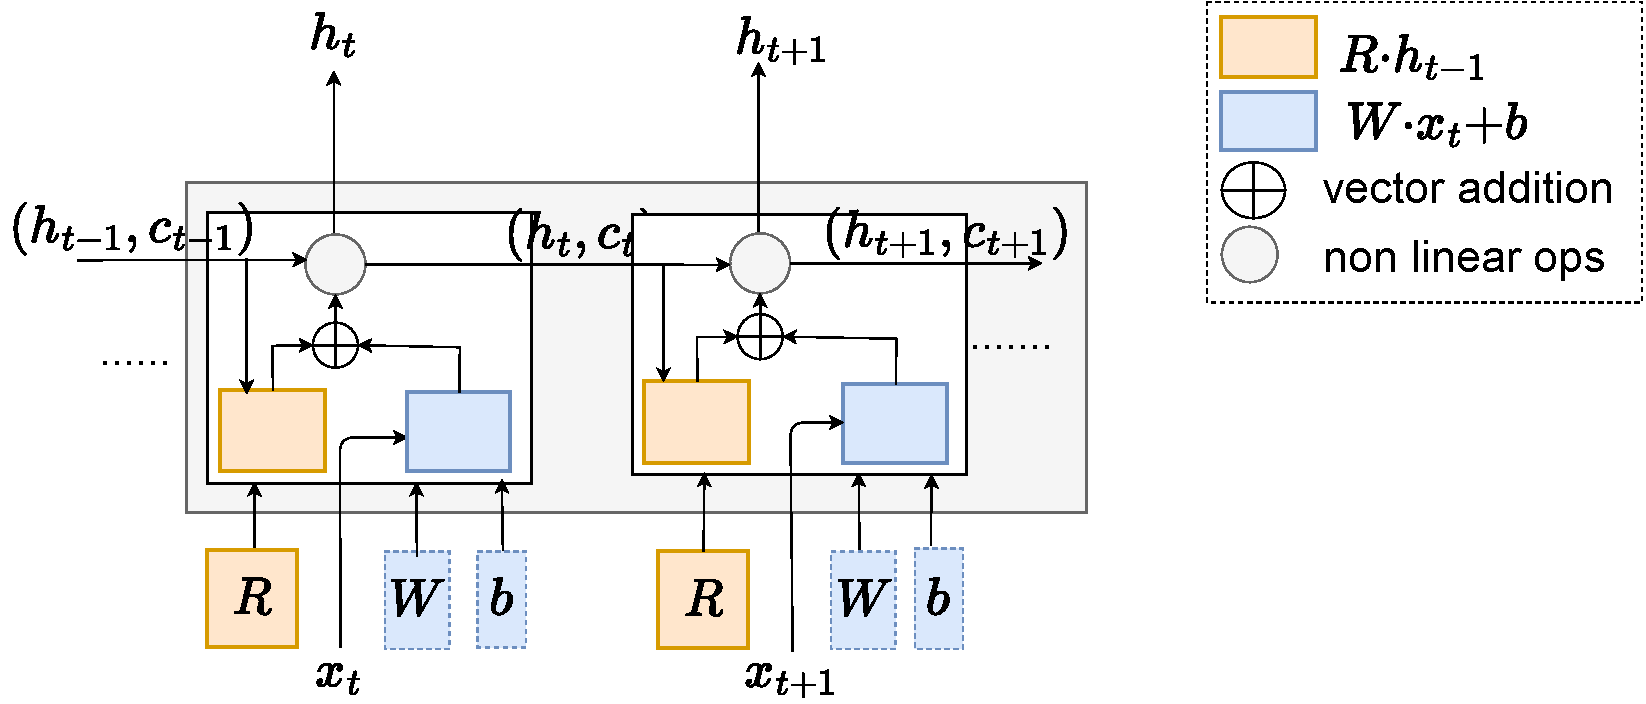
\includegraphics[width=0.7\textwidth]{dataDependencyConventional.pdf}}
	\caption{Data dependency in computations of LSTMs between consecutive time steps}
	\label{fig:lstmComputationConv}
\end{figure}
LSTM computations (~\eqref{eq:lstmEqs}) for two consecutive time steps are shown in~\figurename{~\ref{fig:lstmComputationConv}}. At every time step,~\eqref{eq:lstmEqs} take vectors $x_t$ as input and compute the cell state ($c_t$) and hidden state ($h_t$) using the previous hidden state ($h_{t-1}$) and cell state ($c_{t-1}$) vectors. $h_t$ depends on the present input vector $x_t$ and the previous time step cell state ($c_{t-1}$) and hidden state ($h_{t-1}$) vectors. The dependency of $h_t$ on $h_{t-1}$ and $c_{t-1}$ prevents the parallel processing of multiple time steps. 

LSTM accelerators have small on-chip memory. The large weight matrices $R$ and $W$ are stored in off-chip memory. The dependency of $h_{t}$ and $c_{t}$ on the previous time step computations makes the reuse of weight matrix $R$ a challenge. Thus the weights are accessed from the off-chip memory at every step, resulting in sizeable off-chip memory accesses and high energy consumption of these accelerators. This work focuses on reducing the off-chip memory accesses of $R$ during the LSTM inference phase. 

Our approach splits the computations of a time step and computes the partial sums of two consecutive time steps. As shown in \figurename{~\ref{fig:dataDependencyProposed}}, the proposed approach at time step t computes $h_t$ using the input partial sum $S^U_t$, and partial sum computed at current time step $S^L_t$. $h_t$ is then used to compute the partial sum $S^L_{t{+}1}$ for next time step, while reusing the weights of $R$. $S^L_{t{+}1}$ is then passed for the next step computations of $h_{t{+}1}$. At each time step only half of the matrix $R$ is accessed and reduces the $R$ matrix accesses by half.
\begin{figure}[!htb]
	\centerline{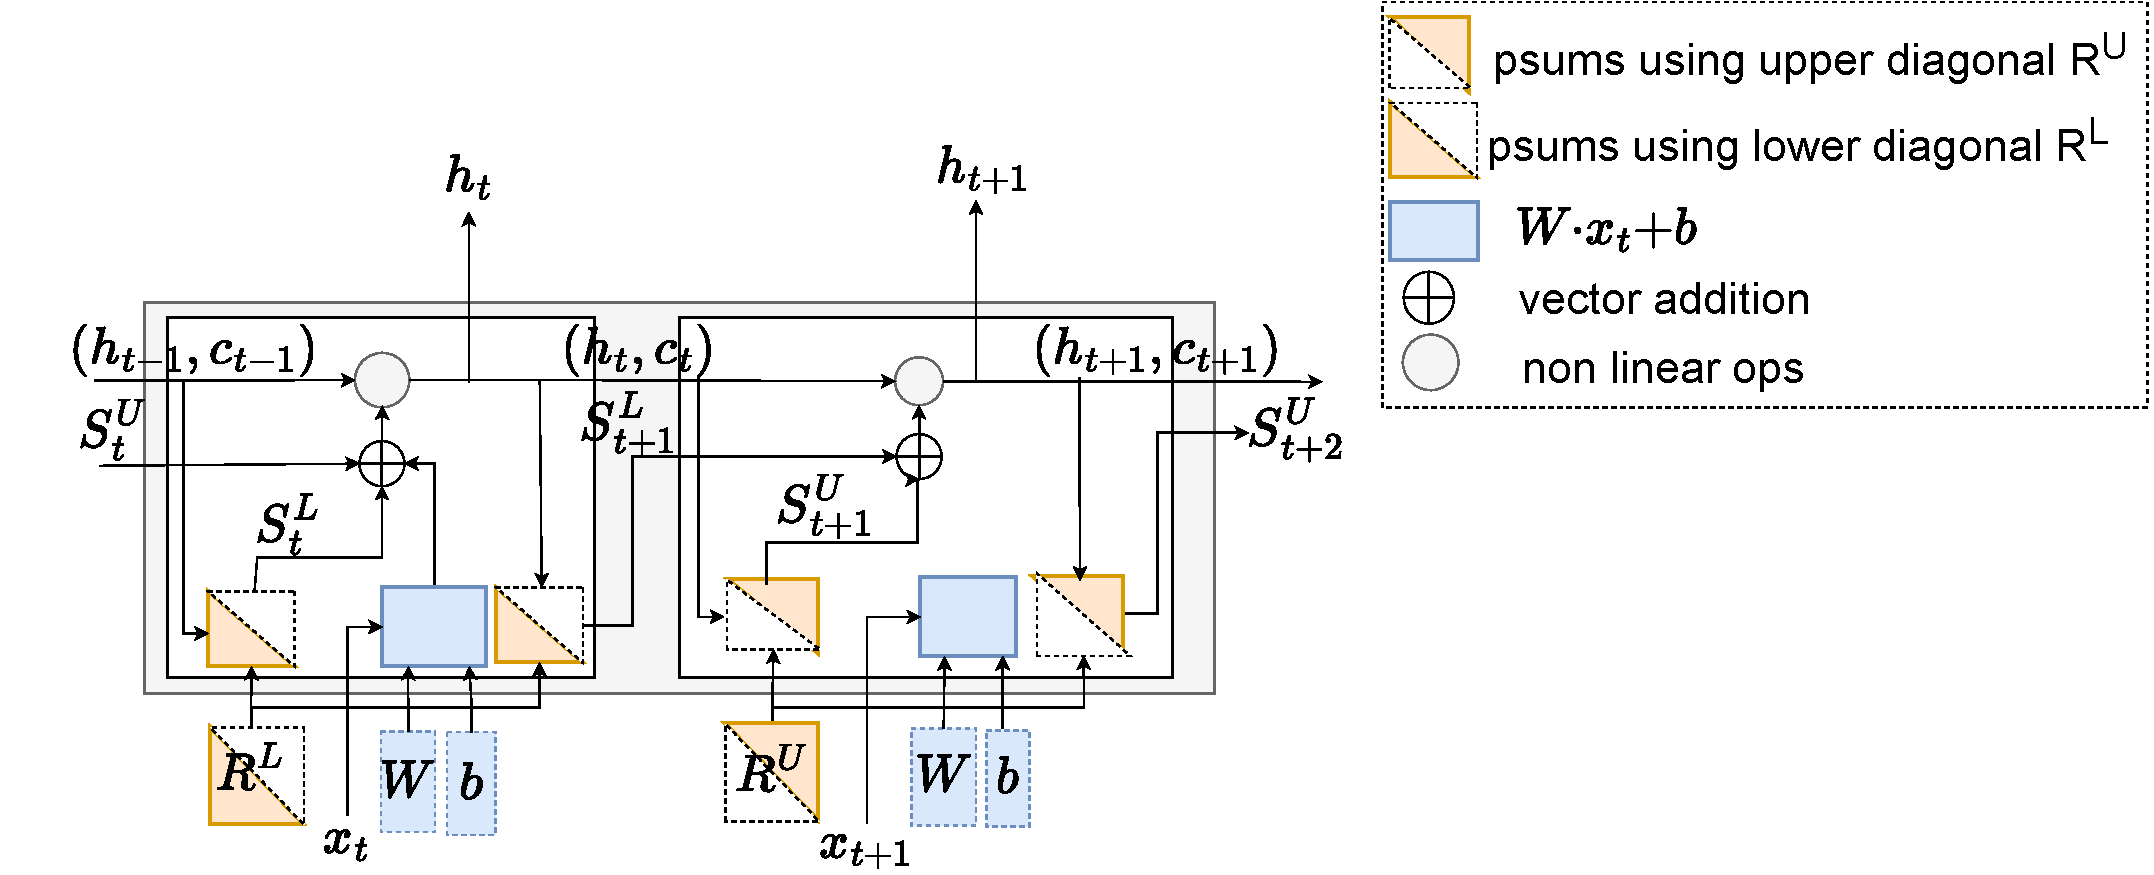
\includegraphics[width=0.85\textwidth]{dataDependencyProposed.pdf}}
	\caption{Proposed approach: Splitting computations into partial sums and reusing the weights of $R$.}
	\label{fig:dataDependencyProposed}
\end{figure}
\section{Related Work}
To address the computational and energy efficiency of LSTMs and in general RNNs, several ASIC~\cite{conti2018chipmunk,wang2017accelerating,azari2020elsa} and FPGA based accelerators~\cite{chang2015recurrent,ferreira2016fpga,lee2016fpga,guan2017fpga,han2017ese} are proposed. The energy efficiency of LSTM accelerators is critical for their widespread usage, and off-chip memory access is the key to improving energy consumption. Most of these works focused on improving energy efficiency by reducing off-chip memory accesses.

Some approaches~\cite{lee2016fpga, rybalkin2018finn, ferreira2016fpga} used on-chip memory to store all the weights. Sizes of weights in recent multi-layer LSTM models can be several MB's, and using large on-chip memory is expensive. These approaches are not scalable and effective only for small LSTM models. Our approach is independent of model size and effective for large LSTM models.

Several approaches used the fact that neural networks are error-tolerant and have lots of redundancy. They used the quantization and pruning techniques to compress the models' size. Approaches~\cite{ferreira2016fpga,wang2018c} used 18-bit, Chang et al.~\cite{chang2015recurrent} used 16-bit, Han et al.~\cite{han2017ese} used 12-bits precision for storing the inputs and weights, Lee et al.~\cite{lee2016fpga} used 8-bit inputs and 6-bits for weights to reduce the model size. Our approach is orthogonal to the quantization techniques and can be integrated with different quantization techniques to reduce the memory accesses further. 

Han et al.~\cite{han2017ese} used pruning to compress the model. However, pruning results in irregular network structure, and the sparse matrices require additional computational and storage resources resulting in unbalanced load distribution. To overcome this Wang et al.~\cite{wang2018c} used block-circulant matrices representations to compress the LSTM/RNN model and to eliminate irregularities resulted from compression. Some approaches~\cite{park2019balancing,han2017ese,park2018maximizing} used load balance aware pruning techniques to overcome the unbalanced load distribution problem. 

Quantization and pruning approaches compromise the accuracy of the networks. The other line of works reduced the memory accesses without effecting the accuracy of the NNs output by applying the data-reuse techniques. The matrix-vector multiplication $W^j{\cdot}x$ in~\eqref{eq:lstmEqs}, where $j\in \{i,f,g,o\}$, is independent of previous state computation. Que et al.~\cite{que2019efficient} proposed a blocking-batching scheme that reuses the weights of $W^j$ matrix by processing a group of input vectors as a batch. The input vectors in the same batch share the same weight matrices ($W^j$). However, it is difficult to collect the required number of input vectors. As the LSTM cell states ($h_t$ and $c_t$) computations depend on previous time-step cell states, the benefit of their batching schemes is limited to $W^j{\cdot}x$. Reusing weights of $R$ across different time steps has not been successful because of the dependency on previous time-step states.

Park et al.(~\cite{park2020time}) proposed a time-step interleaved weight reuse scheme (TSI-WR) which reuses the weights of $R$ matrix between two adjacent time steps by performing computations in a time-interleaved manner. Their approach logically partitions the $R$ matrix into blocks. A block is accessed from off-chip memory to compute the hidden state vector $h_t$, and a fraction of it is reused to compute the partial sum of next time step state $h_{t+1}$. However, their approach does not fully exploit the data reuse, and several weights are accessed repeatedly from the off-chip memory. In addition, the data reuse in the TSI-WR approach depends on the on-chip storage size which benefits accelerators with larger on-chip memory.

Our approach schedules the computations in a way that reuses all the weights of $R$ between two adjacent time steps. The data reuse in our approach is independent of on-chip buffer sizes which even benefits to accelerators with small on-chip memory. 

\section{Split And Combine Computations Approach}
In this section, we first describe basic idea of Split And Combine Computations (\textbf{SACC}) approach and then its extension to block-wise reuse of data.
\subsection{Basic Approach}\label{sec:elementWiseApproach}
The computation of the $h_t$ can be expressed as shown below
\begin{align}\label{eq:h_{t}}
	h_{t}[k] &= F( S_{t}[k]+q_{t}[k])
\end{align}
where $F$ is a non-linear function. $q_{t}$ is computed as $W{\cdot}x_t{+}b$ and its computations are independent of previous step cell states. $S_{t}[k]$ is the sum of $N$ product terms as shown below,
\begin{align}\label{eq:S_{t}}
	S_{t}[k] = \sum_{n=0}^{N-1}R[k][n]\cdot h_{t-1}[n]
\end{align}
Computations of $S_{t}[k]$, and therefore $h_{t}[k]$, depends on all the $N$ elements of $h_{t-1}$. Conventional approaches first compute all the $N$ elements of $h_{t-1}$, which require accessing the full matrix $R$, before initiating the computations of $h_{t}$. Due to limited on-chip memory, elements of matrix $R$ are replaced by other weights of $R$ required for computations of next elements of $h_{t}$. When accelerator starts computing $h_{t+1}$, weights of $R$ are accessed again from the off-chip memory .

To reuse the weights of $R$, we split the computations of \eqref{eq:S_{t}} into the following two partial sums 
\begin{align}\label{eq:S_{t}_split}
	S_{t}[k] = \sum_{n=0}^{k}R[k][n]\cdot h_{t-1}[n] + \sum_{n=k+1}^{N-1}R[k][n]\cdot h_{t-1}[n]
\end{align}
Let $S_{t}^{L}[k]$ and $S_{t}^{U}[k]$ are the first and second partial sums in \eqref{eq:S_{t}_split}, respectively.  $S_{t}^{L}[k]$ and $S_{t}^{U}[k]$ are expressed in equations below, 
\begin{align}
	S_{t}^{L}[k] &= \sum_{n=0}^{k}R[k][n]\cdot h_{t-1}[n] \label{eq:S_L_{t}}\\
	S_{t}^{U}[k] &= \sum_{n=k{+}1}^{N-1}R[k][n]\cdot h_{t-1}[n] \label{eq:S_U_{t}}
\end{align}
\eqref{eq:S_L_{t}} uses the lower-diagonal and diagonal elements of $R$ ($R^L$), and~\eqref{eq:S_U_{t}} uses the upper diagonal elements of $R$ ($R^U$). \figurename{~\ref{fig:LowerDiagR}} and \figurename{~\ref{fig:UpperDiagR}} shows the elements of $R$ used in the partial sum computations of $S_{t}^{L}$ and $S_{t}^{U}$, respectively for a $3\times3$ matrix $R$. Each element of $S$ is a sum of three product terms. Partial sum vectors $S^L_t$ and $S^U_t$ have only a fraction of the total sum $S$. The fraction of the sum in each element of $S^L_t$ and $S^U_t$ are highlighted using colored rectangles in \figurename{~\ref{fig:partialSumComputations}}.
\begin{figure}[htb!]
	\centering
	\subfloat[]
	{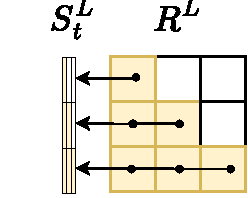
\includegraphics[width=0.3\textwidth]{LowerDiagR.pdf}
		\label{fig:LowerDiagR}}
	\hspace{2.0em}
	\subfloat[]
	{
		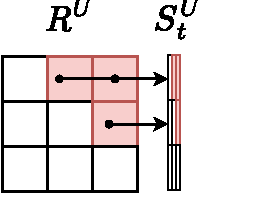
\includegraphics[width=0.3\textwidth]{UpperDiagR.pdf}
		\label{fig:UpperDiagR}
	}
	\caption{Fraction of partial sums computated using (a) lower diagonal element of $R$  (b) upper diagonal elements of $R$ }
	\label{fig:partialSumComputations}
\end{figure}

The elements of $R$ used in the computations of $S_{t}$ are also required for the partial sum computations of $S_{t{+}1}$, as shown below
\begin{align}
	S_{t{+}1}^{L}[k] &= \sum_{n=0}^{k}R[k][n]\cdot h_{t}[n] \label{eq:S_L_{t+1}}\\
	S_{t{+}1}^{U}[k] &= \sum_{n=k{+}1}^{N-1}R[k][n]\cdot h_{t}[n] \label{eq:S_U_{t+1}}
\end{align}
The partial sum $S_{t{+}1}^{L}[k]$ (\eqref{eq:S_L_{t+1}}) depends on the first $k{+}1$ elements of $h_{t}$ and the second partial sum $S_{t{+}1}^{U}[k]$ (\eqref{eq:S_U_{t+1}}) depends on the remaining $N{-}(k{+}1)$ elements of $h_{t-1}$. $S_{t{+}1}^{L}[k]$ computations can be initated soon after first $k{+}1$ elements of $h_{t}$ are computed. Similarly at the next time step, the computations of $S^U_{t{+}2}[k]$ can be initiated soon after the last $N{-}(k{+}1)$ elements of $h_{t{+}1}$ are computed. 

Dividing the computations into two partial sums gives opportunity to reuse the weights of matrix $R$ between two consecutive time steps. In our approach, we access the weights of $R$ and reuse it for computations of partial sums for two consecutive time steps.
%Later, when the remaining $N{-}(k{+}1)$ elements of $h_{t}$ are computed, the partial sum $S_{t{+}1}^{U}[k]$ is computed to finally compute the sum $S_{t{+}1}[k]$, and $h_{t{+}1}[k]$. 

%\begin{figure}[!tb]
%	\centerline{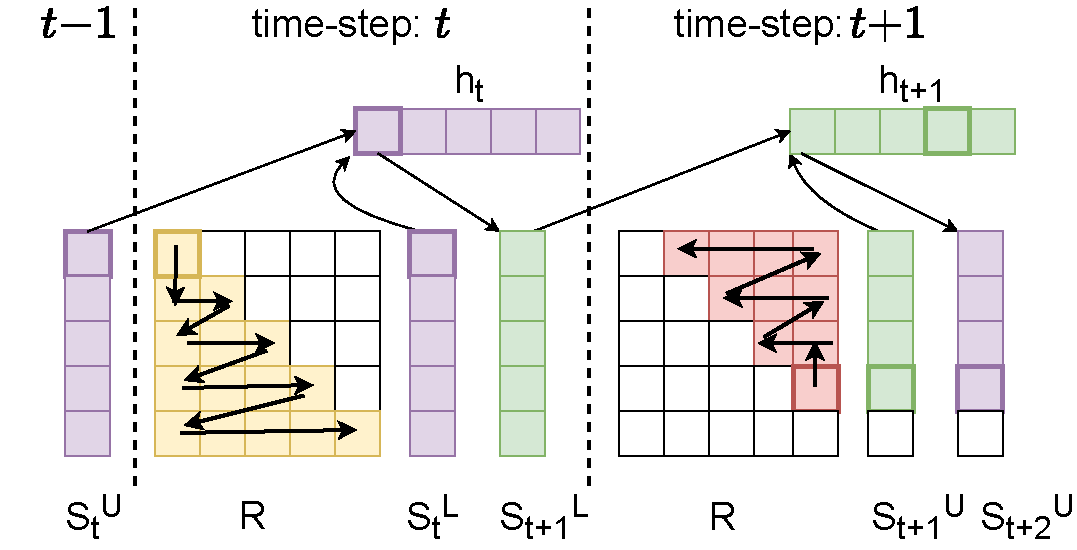
\includegraphics[width=0.33\textwidth]{TwoTimeSteps.pdf}}
%	\caption{Splitting the hidden state vector computations into partial sums}
%	\label{fig:TwoTimeStepsComputation}
%\end{figure}
%Elements of $R^L$ are accessed from top to bottom, left to right, while elements of $R^U$ are accessed in the reverse order to satisfy the dependencies. 

%As shown in \figurename{~\ref{fig:dataDependencyProposed}}, weights of $R^L$ and $R^U$ are reused in the partial sum computations of two steps. At time step $t$, $S_t^U$ and $h_{t-1}$ are the inputs from the previous time step, and $R^L$ is used to compute the partial sums $S_{t}^{L}$ and then added to $S_{t}^{U}$ to compute elements of $h_{t}$. Computed elements of $h_{t}$ are then immediately used to compute elements of  $S_{t+1}^L$. $S_{t+1}^L$ is then passed to $(t{+}1)^{th}$ step computations. In the same way, at time step $t{+}1$, weights of $R^U$ are reused to compute $S_{t+1}^{U}$ and $S_{t+2}^{U}$.  
\begin{comment}
\begin{figure*}[htbp]
	\centerline{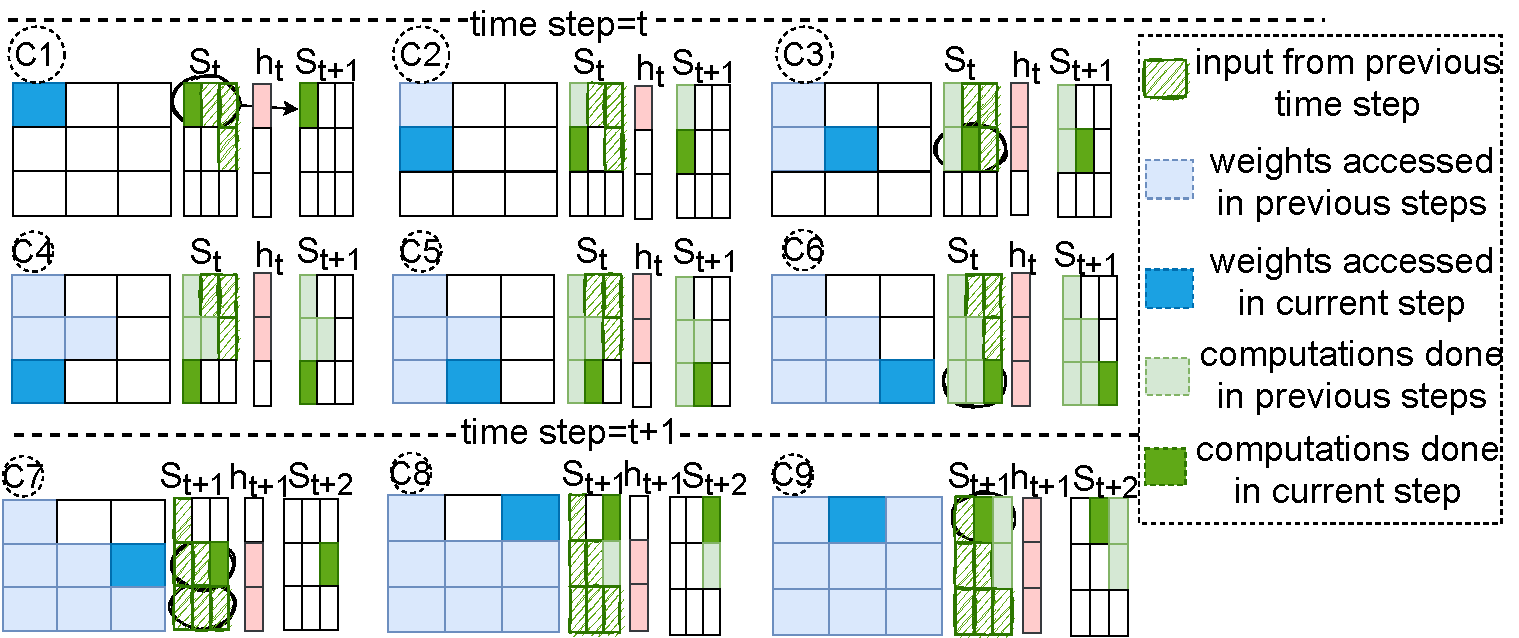
\includegraphics[width=0.9\textwidth]{proposedWithInit_withH.pdf}}
	\caption{Computation of consecutive hidden state vectors $h_1$, $h_2$ and $h_3$ while accessing $R$ matrix from off-chip memory.}
	\label{fig:ExampleComputation}
\end{figure*}
\figurename{~\ref{fig:ExampleComputation}} illustrates the compute-steps (C1 to C9) and weights accessed for computing the outputs of two time steps for $N{=}3$. The shaded rectangular blocks shows the product terms input from the previous time step ($t{=}1$). When all the product terms ($R[k][j]{\cdot}h_{t-1}[j]$) for the partial sum vector  element ($S_t[k]$) are computed, then $h_t[k]$ is computed (shown as pink blocks in \figurename{\ref{fig:ExampleComputation}}). The weights of $R$ are reused for the product terms $R[k][j]{\cdot}h_{t}[j]$ for computing the partial sum $S_{t+1}$, using the values of $h_t$ computed in previous or present compute-step. As shown in \figurename{\ref{fig:ExampleComputation}} matrix $R$ is accessed in 9 compute-steps ($N{\times}N$) to compute $h_t$ and $h_{t+1}$ and the partial sum $S_{t+2}$ for the next time step ($t{+}1$).
\end{comment}
\begin{figure}[htbp]
	\centerline{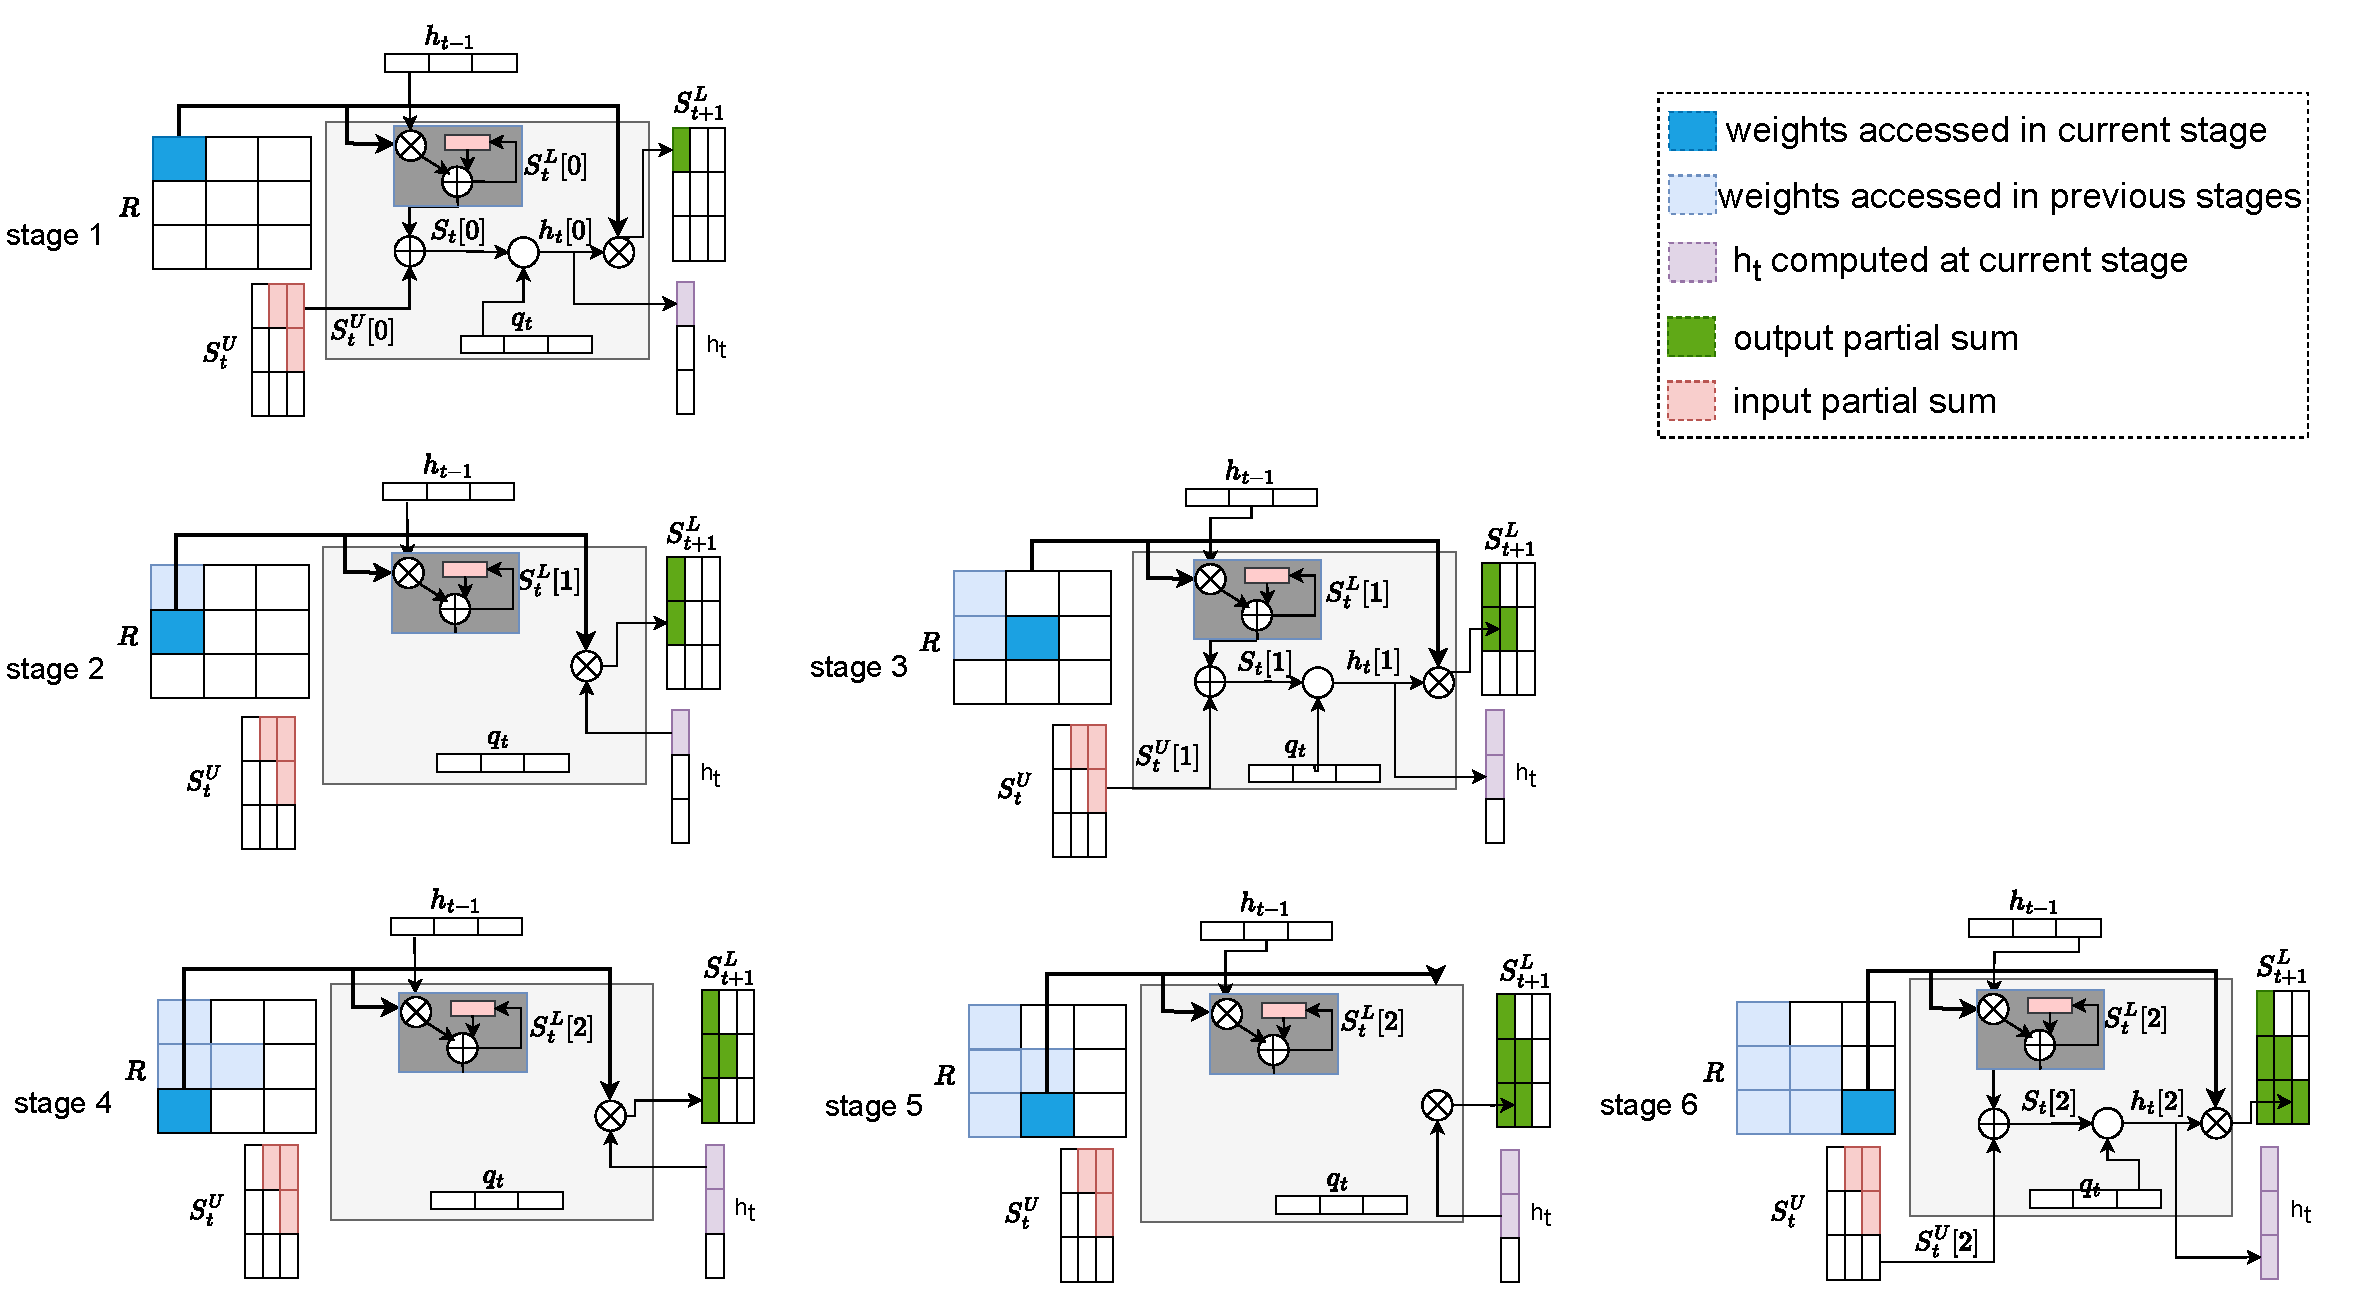
\includegraphics[keepaspectratio=true, width=\textwidth]{LSTMStepStages_t.pdf}}
	\caption{Computation steps (stages) at time step $t$ for computing hidden state vectors $h_t$ and partial sum $S^L_{t{+}1}$ while accessing $R^L$.}
	\label{fig:ExampleComputation_t}
\end{figure}
\begin{figure}[htbp]
	\centerline{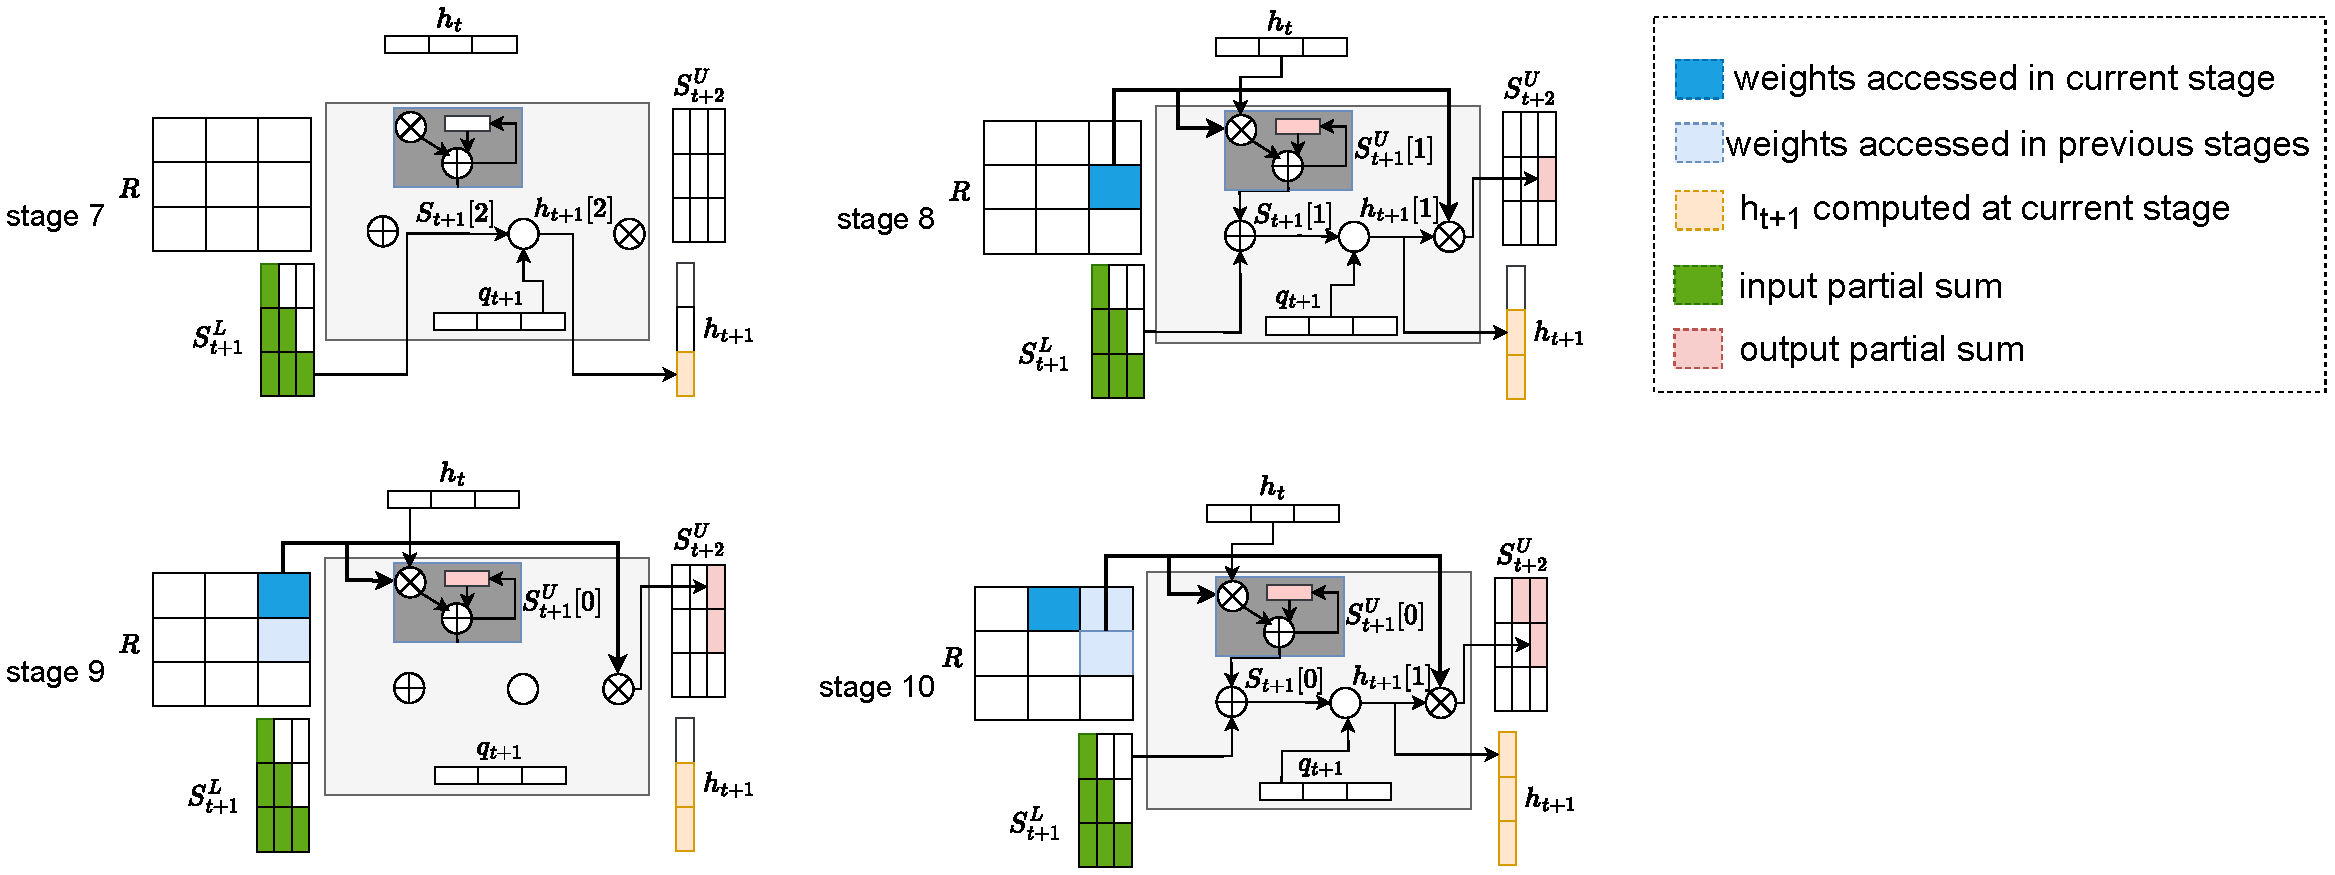
\includegraphics[keepaspectratio=true,width=\textwidth]{LSTMStepStages_t1.pdf}}
	\caption{Computation steps (stages) at time step $t{+}1$ for computing hidden state vectors $h_{t+1}$ and partial sum $S^U_{t{+}2}$ while accessing $R^U$.}
	\label{fig:ExampleComputation_t+1}
\end{figure}
An example to describe different stages of computations performed in two consecutive steps $t$ and $t{+}1$ is shown in \figurename{~\ref{fig:ExampleComputation_t}} and \figurename{~\ref{fig:ExampleComputation_t+1}} , respectively, for a $3{\times}3$ matrix $R$.  The reuse of weights of $R$ at different stages are shown in bold lines in  \figurename{~\ref{fig:ExampleComputation_t}} and \figurename{~\ref{fig:ExampleComputation_t+1}}.

There are 6 stages at time step $t$. At each stage an element of $R$ is accessed and passed as input to a multiply accumlate unit (MAC) that multiplies the element of $R$ with an element of $h_{t{-}1}$ and accumlates the product terms, until all the elements of a row of $R^L$ are accessed. After that output of MAC is passed to an adder to perform the addition with corresponding element of $S^U_{t}$ and accumlater is reset to zero. At stage 1, $R[0][0]$ is accessed, and the product $S^L_t[0]{=}R[0][0]{\cdot}h_{t{-}1}[0]$ is computed. $S^L_t[0]$ is then added to the input partial sum $S^U_t[0]$ to compute sum $S_t[0]$. $S_t[0]$ is used to compute $h_t[0]$ using \eqref{eq:h_{t}} and $h_t[0]$ is then immediately used to compute $S^L_{t{+}1}[0]$ while reusing the weight $R[0][0]$. 

Stage 2 and Stage 3 access the weight $R[1][0]$ and $R[1][1]$, respectively to compute $h_t[1]$ and the partial sum $S^L_{t{+}1}[1]$. At stage 2, $R[1][0]$ is multiplied with $h_{t{-}1}[0]$ to update $S^L_t[1]$. $R[1][0]$ is then reused to compute the product term $R[1][0]{\cdot}h_t[0]$, using $h_t[0]$ computed at stage 1. At stage 3, $R[1][1]$ is multiplied with $h_{t{-}1}[1]$ and added to $S^L_{t{+}1}[1]$ computed at stage 2, to get the partial sum $S^L_t[1]$. $S^L_t[1]$ is then passed to the adder which adds it to the input $S^U_t[1]$ to compute $S_t[1]$. $S_t[1]$ is used to compute $h_t[1]$ using \eqref{eq:h_{t}}. $h_t[1]$ is then immediately used to compute $S^L_{t{+}1}[1]$, while reusing the weight $R[1][1]$.

Similarly, stage 4, stage 5 and stage 6 reuse weights of $R^L[2]$ to compute $h_t[2]$ and the partial sum $S^L_{t{+}1}[2]$. At time step $t$, $h_t$ and the partial sum $S^L_{t{+}1}$ is computed which are used as input to the next time step $t{+}1$.
 
\figurename{~\ref{fig:ExampleComputation_t+1}} shows the computation stages for $t{+}1$. At time step $t{+}1$, inputs are $h_t$ and partial sum $S^L_{t{+}1}$, and computes the output $h_{t{+}1}$ and the partial sum $S^U_{t{+}2}$. Together in \figurename{~\ref{fig:ExampleComputation_t}} and \figurename{~\ref{fig:ExampleComputation_t+1}}, accesses all the elements of $R$ once to compute the outputs $h_t$ and $h_{t{+}1}$ and a partial sum $S^U_{t{+}2}$ which is passed to next time step. 

\subsection{Block-wise reuse}
%\begin{figure}[!tb]
%	\centerline{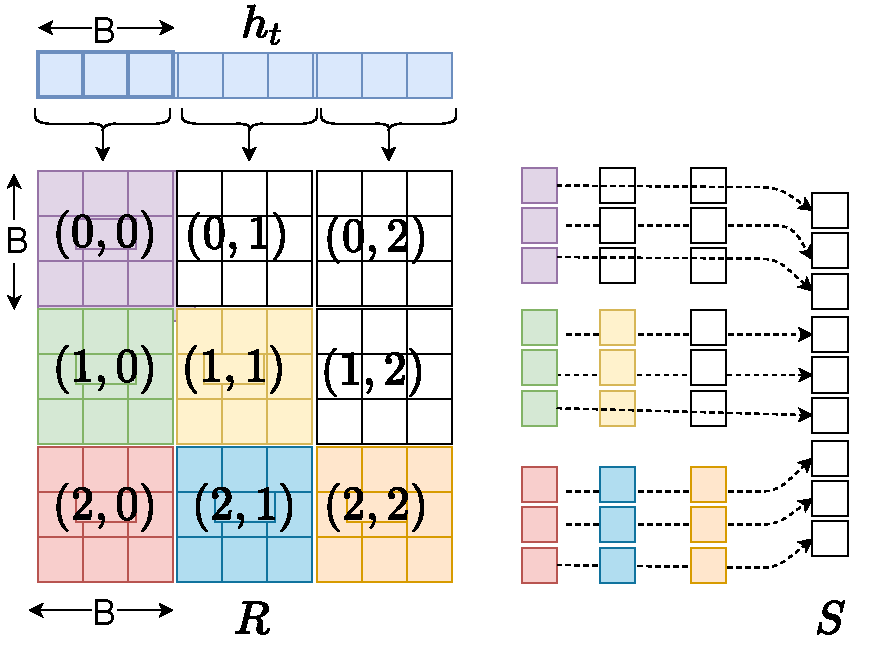
\includegraphics[width=0.5\textwidth]{blockApproachA.pdf}}
%	\caption{Partitions of $R$ in $B{\times}B$ blocks and partial sum computations.}
%	\label{fig:blockApproach}
%	\vspace{-1.0em}	
%\end{figure}
The basic approach accesses one elements of $R$ at each stage. LSTM accelerator can store several elements of $R$. To process several element of $R$, the basic approach can be extended by partitioning $R$ into square matrices. The size of the square matrices is determined by the available on-chip memory of the accelerator. Let $R$ is partitioned into square matrices $P$ of size $B{\times}B$, such that $P$ fits in the accelerator's on-chip memory. Each $P$ matrix can be indexed as $(r,m)$, where $0{\le}r,m{\le} (\ceil{\frac{N}{B}}{-}1)$, as shown in \figurename{~\ref{fig:squareMatrix}}. We group these small matrices into $R^L$ and $R^U$ such that $R^L$ has all the matrices with index $r{\geq}m$  and $R^U$ has all the matrices with index $r{<}m$, as shown in \figurename{~\ref{fig:lowerSquareMatrix}} and \figurename{~\ref{fig:upperSquareMatrix}}, respectively.
\begin{figure}[htb!]
	\centering
	\subfloat[]
	{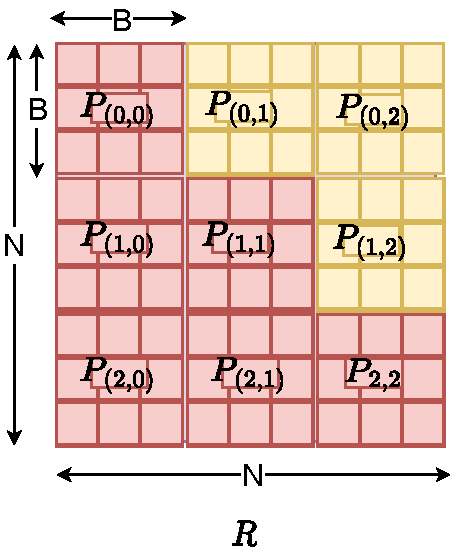
\includegraphics[width=0.25\textwidth]{squareMatrix.pdf}
		\label{fig:squareMatrix}}
%	\hspace{2.0em}
	\subfloat[]
	{
		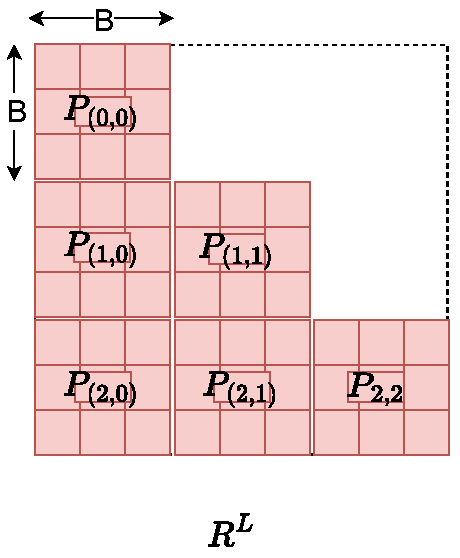
\includegraphics[width=0.25\textwidth]{lowerSquareMatrix.pdf}
		\label{fig:lowerSquareMatrix}
	}
	\subfloat[]
	{
		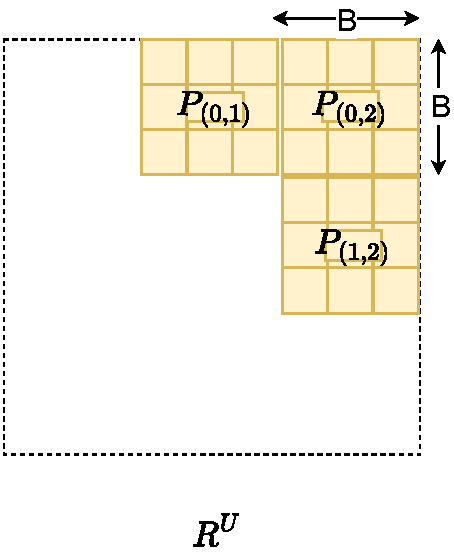
\includegraphics[width=0.245\textwidth]{upperSquareMatrix.pdf}
		\label{fig:upperSquareMatrix}
	}
	\caption{(a) Partitions of a matrix $R_{N{\times}N}$ into $B{\times}B$ square matrices $P_{(r,m)}$ (b) $R^L{=}\{P_{(r,m)}:r{\geq}m$\} (b) $R^U{=}\{P_{(r,m)}:r{<}m$\}	}
	\label{fig:SquareMatrices}
	\vspace{-1.0em}	
\end{figure} 

In block approach, we divide the computations of $h_t$ into $(\ceil{\frac{N}{B}}{-}1)$ slices, each such slice having $B$ elements. \figurename{~\ref{fig:hVectorSlices}} shows an example vector $h_t$ of length $N{=}9$, divided into slices of length $B{=}3$. $r^{th}$ slice of $h_t$ require all the partitions $P_{r{\times}m}$ having the same row index $r$. Partitions $P$ used in the computations of each slice of $h$ are also shown under each slice in \figurename{~\ref{fig:hVectorSlices}}. Computed values of $h_t$ are then immediately used to compute the partial sum for the next time step while reusing the weights of partitions $P$.  
\begin{figure}[!htb]
	\centerline{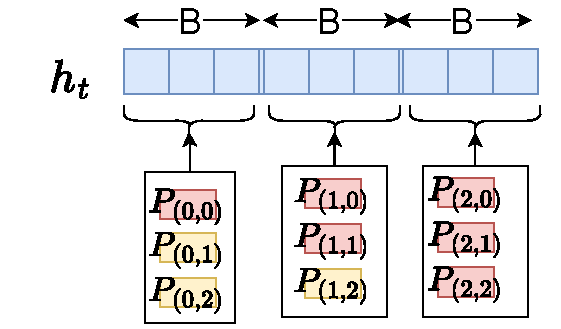
\includegraphics[width=0.4\textwidth]{hVectorSlices.pdf}}
	\caption{Slices of vector $h$ and partitions of $R$ required to compute each slice of $h$.}
	\label{fig:hVectorSlices}
	\vspace{-1.0em}	
\end{figure}

$k^{th}$ element of $r^{th}$ slice of $h_{t}$ can be computed as following, where $0{\le}k{\le}B{-}1$. 
\begin{align}
	h_{t}[B{*}r{+}k]{=}F(\sum_{m{=}0}^{\ceil{\frac{N}{B}}{-}1}S_{(r,m)}[k]+q_{t}[B{*}r{+}k]) \label{eq:blockWiseh}
\end{align}
where $S_{(r,m)}$ is the partial sum of the $r^{th}$ slice of $S$, computed using the partition $P_{(r,m)}$, and $S_{(r,m)}[k]$ is the $k^{th}$element of $S_{(r,m)}$ vector that can be computed using the equation below,
\begin{align}	 \label{eq:blockWiseSum}
	\begin{split}
	S_{(r,m)}[k]&{=}\sum_{j=0}^{B{-}1}P_{(r,m)}[k][j]\cdot h_{t-1}[B{*}m{+}j]\\
	&{=}\sum_{j=0}^{B{-}1}R[B{*}r{+}k][B{*}m{+}j]\cdot h_{t-1}[B{*}m{+}j]
 \end{split}
\end{align}
The summation $\sum_{m{=}0}^{\ceil{\frac{N}{B}}{-}1}S_{(r,m)}[k]$ in~\eqref{eq:blockWiseh} can be split as following partial sums
\begin{align}
	&\sum_{m{=}0}^{\ceil{\frac{N}{B}}{-}1}S_{(r,m)}[k]{=}\sum_{m{=}0}^{r}S_{(r,m)}^{L}[k]{+}\sum_{m{=}r{+}1}^{\ceil{\frac{N}{B}}{-}1}S_{(r,m)}^{U}[k] 
\end{align}
\begin{figure}[!htb]
	\centerline{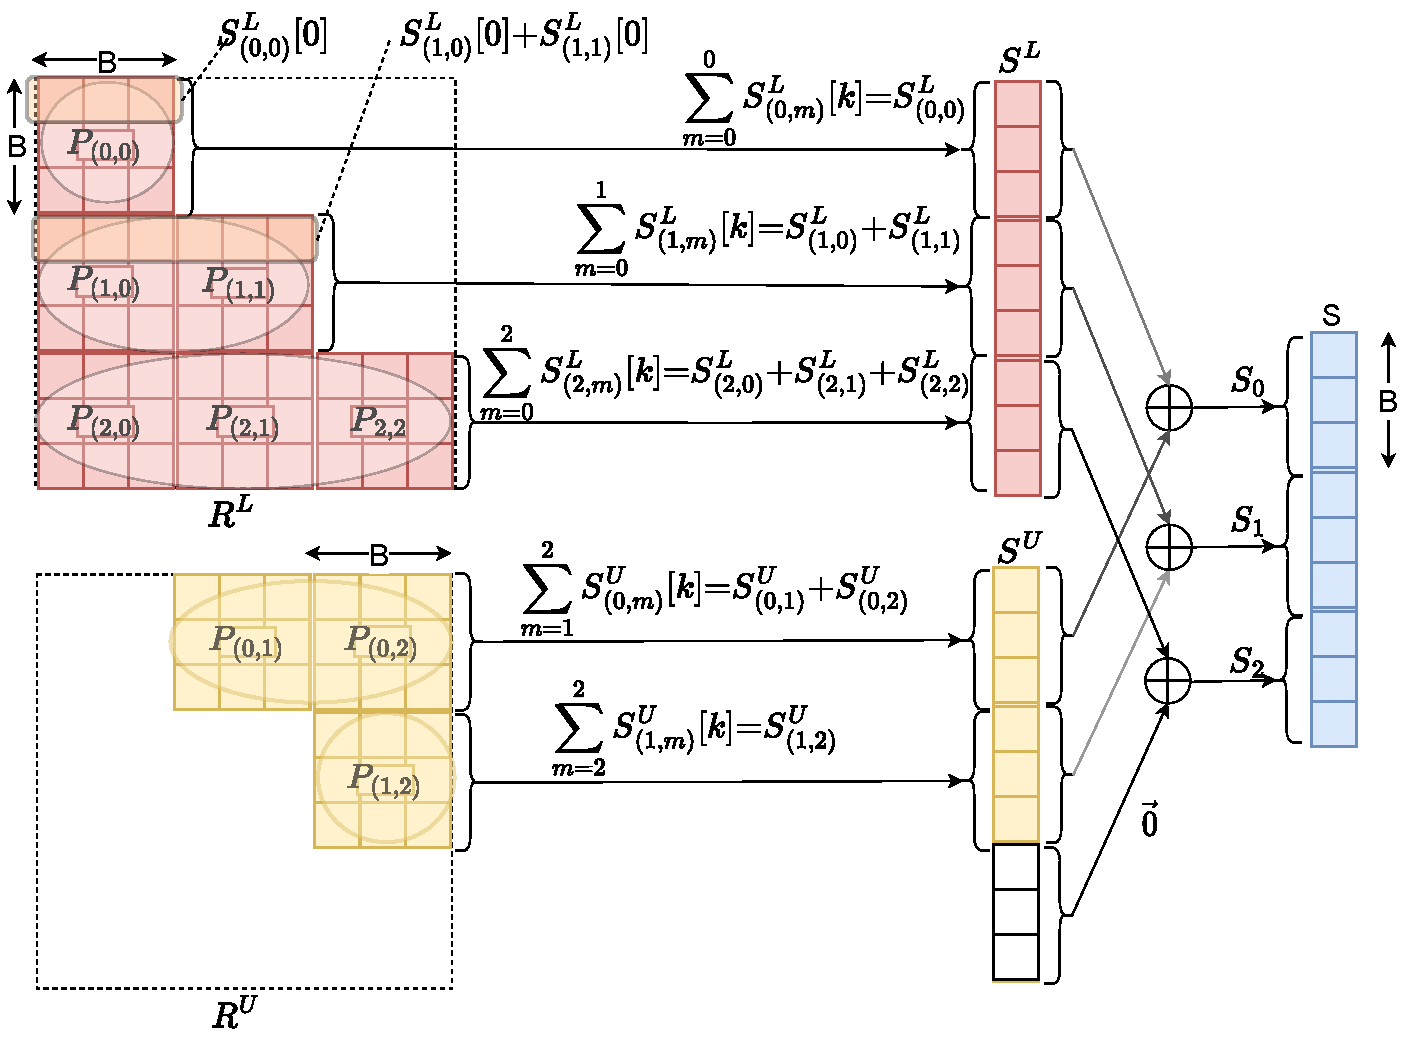
\includegraphics[keepaspectratio=true,width=0.7\textwidth]{blockPartialSum.pdf}}
	\caption{Partitions $P_{(r,m)}$ of $R^L$ and $R^U$ required for computations of partial sum $S^L$ and $S^U$.}
	\label{fig:blockPartialSum}
	\vspace{-1.0em}	
\end{figure}

$\sum_{m{=}0}^{r}S_{(r,m)}^{L}[k]$ uses the partitions $P$ from $R^L$ (\figurename{~\ref{fig:lowerSquareMatrix}}), and $\sum_{m{=}r{+}1}^{\ceil{\frac{N}{B}}{-}1}S_{(r,m)}^{U}[k]$ uses partitions $P$ from $R^U$ (\figurename{~\ref{fig:upperSquareMatrix}}). \figurename{~\ref{fig:blockPartialSum}} describes the partitions $P$ used in the computation of $\sum_{m{=}0}^{r}S_{(r,m)}^{L}[k]$ and $\sum_{m{=}r{+}1}^{\ceil{\frac{N}{B}}{-}1}S_{(r,m)}^{U}[k]$.

Partial sum computations of $r^{th}$ slice of $(t{+}1)^{th}$ time step can be initiated as soon as the first $r$ slices ($B{\times}r$ elements) of $h_t$ are computed.
Computations of the $r^{th}$ slice of partial sums ($S_L$ and $S_U$) at different time steps, use the same partitions $P$ of $R$. Our approach exploits this to reuse the weights of $P$ for the computations of partial sums of two consecutive time step, as shown in \figurename{~\ref{fig:dataDependencyProposed}}. 

Algorithm~\ref{Algo:SACCAlgo} describes the block wise SACC approach. The dimensions of $W$, $R$, $b$, and $x_t$ are $4N{\times}L$, $4N{\times}N$, $4N{\times}1$, and $L{\times}1$, respectively. The algorithm stores the vectors $h_t$, $c_t$, and the partial sum vectors ($s_{t+1}$) in the on-chip memory and accesses the weights from the off-chip memory. It first computes the vector $q_t$ as $W{\cdot}x{+}b$, at line~\ref{alg:Wx+b} and then invokes the procedures $\textproc{UpDiagReuse}$ at line~\ref{alg:callUpDiaReuse} or  \textproc{LowDiagReuse} at line~\ref{alg:callLowDiaReuse} at alternate time steps. \textproc{LowDiagReuse} accesses blocks of $R^L$, and \textproc{UpDiagReuse} accesses blocks of $R^U$. The procedures have two nested loops. \textproc{LowDiagReuse} traverses the blocks from top to bottom (at line \ref{alg:LowDiag_outFor}), left to the right (at line \ref{alg:LowDiag_inFor}), while the \textproc{UpDiagReuse} traverses the blocks in the opposite order. The inner loop accesses the $(r,m)^{th}$ block of $R$ from the off-chip memory and reuses it to compute the partial sums $s^B_{t+1}$ and $s^B_{t+2}$. The outer loop iterations compute $r^{th}$ slices of $h_{t+1}$, $c_{t+1}$, and $s_{t+2}$.
When all the blocks of the $r^{th}$ row are processed, $s^B_{t+1}$ has the total sum, which is then used to compute the $r^{th}$ slice of the vectors $h_{t+1}$ and $c_{t+1}$ using \textproc{LSTMEquations} at line~\ref{alg:LowDiag_LstmEq}. 
Both the procedures reuse the blocks of $R$ to reduce the off-chip memory accesses. Algorithm~\ref{Algo:LSTMEq} implements the LSTM equations using the partial sum vector.
\begin{algorithm}[H]
	\caption{SACC algorithm}
   \label{Algo:SACCAlgo}
	\begin{algorithmic}[1]
		\Procedure{CompLSTMCell}{$W$,$R$,$b$,$x_{t+1}$} \label{alg:CompLSTMCell}
\State $q_{t+1}\gets \Call{MxV}{W,x_{t+1},4N,L}{+}b$\label{alg:Wx+b}
\If{($stage$ is even)}
\State $(h_{t},c_{t},s_{t+1}){\gets}\Call{UpDiaReuse}{R,q_t,h_t,c_t,s_{t+1}}$\label{alg:callUpDiaReuse}
\State $stage\gets odd$
\Else
\State $(h_{t},c_{t},s_{t+1}){\gets}\Call{LowDiaReuse}{R,q_t,h_t,c_t,s_{t+1}}$\label{alg:callLowDiaReuse}
\State $stage\gets even$
\EndIf
%\State ($h_{t},c_{t},s_{t+1})\gets (h_{t+1},c_{t+1},s_{t+2})$
\State \textbf{return} $(h_{t})$
\EndProcedure	
%	\end{algorithmic}
%\end{algorithm}
%
%\begin{algorithm}[ht]
%	\caption{SACC algorithm}
%   \label{Algo:BlockReuse}
%	\begin{algorithmic}[1]
%		\Procedure{Init}{}
%		\State$s_{t+1}\gets \vec{0}$\Comment{partial sum}
%		\State ($h_{t},c_{t}){\gets} (\vec{0},\vec{0})$\Comment{LSTM cell state}
%		\State $stage{\gets} even$
%		\EndProcedure				
		\Procedure{LowDiagReuse}{$R,q_t,h_t,c_t,s_{t+1}$} \label{alg:LowDiagReuse}
		\For {$r\leftarrow 0~\textbf{to}~(\ceil{\frac{N}{B}}{-}1)$} \label{alg:LowDiag_outFor} 
		\State $(i_s,i_e) \gets (r{\cdot}B,(r{+}1){\cdot}B{-}1), s^B_{t+2} \gets \vec{0}$
%		\State $s^B_{t+2} \gets \vec{0}$
		\For {$m \leftarrow 0~\textbf{to}~r$} \label{alg:LowDiag_inFor}
		\State $\textbf{R}^B {\gets}\Call{getDDRBlks}{R,r,m,B}$	     \label{alg:LowDiag_GetDDRBlks}   		     
       \State $(h^B_t,c^B_t,q^B_t)\gets \Call{GetSlice}{h_t,c_t,q_t,m}$ \label{alg:LowDiag_GetSlice}
       \State $s^B_{t+1}\gets \Call{GetSlices}{s_{t+1},m}$ \label{alg:LowDiag_GetSlices}
		\State $s^B_{t+1}\gets s^B_{t+1}{+}\Call{MxV}{\textbf{R}^B,h^B_t,4B,B}$ \label{alg:LowDiag_ReuseR1}  
		
		%\Comment{if diagonal block}
		\If{$m=r$} \label{alg:LowDiag_if}
		\State$(h^B_{t+1},c^B_{t+1}){\gets}\Call{lstmEqns}{v^B_x,s^B_{t+1},c^B_t}$ \label{alg:LowDiag_LstmEq} 
		\State $h_{t+1}\left [i_s\colon i_e\right ]\gets h^B_{t+1}, c_{t+1}\left [i_s\colon i_e\right ]\gets c^B_{t+1}$ \label{alg:LowDiag_UpdateH} 
%		\State $c_{t+1}\left [i_s\colon i_e\right ]\gets c^B_{t+1}$\label{alg:LowDiag_UpdateC}
		\EndIf

		\State $h^B_{t+1}\gets h_{t+1}\left [m{\times}B\colon (m{+}1){\times}B{-}1\right ]$
		\State $s^B_{t+2}\gets s^B_{t+2}{+}\Call{MxV}{\textbf{R}^B,h_{t+1}^B, 4B,B}$  \label{alg:LowDiag_ReuseR2}  
		\EndFor
		\State $s_{t+2}\gets \Call{updateVect}{s_{t+2},s_{t+2}^B,r}$
		\EndFor
		\State \textbf{return} $(s_{t+2},h_{t+1},c_{t+1})$	
		\EndProcedure
		
		\Procedure{UpDiagReuse}{$R,q_t,h_t,c_t,s_{t+1}$}\label{alg:UpDiagReuse}
		\For {$r\leftarrow (\ceil{\frac{N}{B}}{-}1)~\textbf{downto}~0$}\label{alg:UpDiag_outFor} 
		\State $(i_s,i_e) \gets (r{\cdot}B,(r{+}1){\cdot}B{-}1),  s^B_{t+2} \gets \vec{0}$
%		\State $s^B_{t+2} \gets \vec{0}$
		
		\For {$m \leftarrow (\ceil{\frac{N}{B}}){-}1~\textbf{downto}~r{+}1$} \label{alg:UpDiag_inFor} 
		\State $\textbf{R}^B {\gets}\Call{getDDRBlks}{R,r,m,B}$ \label{alg:UpDiag_GetDDRBlks}   
       %\State $(h^B_t,c^B_t,q^B_t,s^B_{t+1})\gets \Call{GetOnChipVecSlice}{h_t,c_t,q_t,s_{t+1},m}$
        \State $(h^B_t,c^B_t,q^B_t)\gets \Call{GetSlice}{h_t,c_t,q_t,m}$ \label{alg:UpDiag_GetSlice}
        \State $s^B_{t+1}\gets \Call{GetSlices}{s_{t+1},m}$ \label{alg:UpDiag_GetSlices}
 
		\State $s^B_{t+1}\gets s^B_{t+1}{+}\Call{MxV}{\textbf{R}^B,h^B_t,4B,B}$\label{alg:UpDiag_ReuseR1} 
		\State $h^B_{t+1}\gets h_{t+1}\left [i_s\colon i_e\right ]$
		\State $s^B_{t+2}\gets s^B_{t+2}{+}\Call{MxV}{\textbf{R}^B,h_{t+1}^B, 4B,B}$; \label{alg:UpDiag_ReuseR2}   
		\EndFor
		
		\State$(h^B_{t+1},c^B_{t+1}){\gets}\Call{lstmEqns}{v^B_x,s^B_{t+1},c^B_t}$ \label{alg:UpDiag_LstmEq}
		\State $h_{t+1}\left[i_s\colon i_e\right ]\gets h^B_{t+1}, c_{t+1}\left[i_s\colon i_e\right ]\gets c^B_{t+1}$ \label{alg:UpDiag_UpdateH}
%       \State $c_{t+1}\left [i_s\colon i_e\right ]\gets c^B_{t+1}$\label{alg:UpDiag_UpdateC}
		\State $s_{t+2}\gets \Call{updateVect}{s_{t+2},s_{t+2}^B,r}$        
		\EndFor    
		\State \textbf{return} $(s_{t+2},h_{t+1},c_{t+1})$	
		\EndProcedure
	\end{algorithmic}
\end{algorithm}

\begin{algorithm}[h]
	\caption{LSTM Equations}
   \label{Algo:LSTMEq}
	\begin{algorithmic}[1]
		\Procedure{lstmEqns}{$q_{t+1},s_{t+1},c_t$}
		\State $(v_i,v_f,v_g,v_o)\gets ExtractVecs(q_t,B)$
		\State $(s_i,s_f,s_g,s_o)\gets ExtractVecs(s_{t+1},B)$
		\For{$n\leftarrow 0~\textbf{to}~B{-1}$}
		\State $i[n]\gets \Call{sigmoid}{s_i[n]+ v_i[n]}$
		\State $f[n]\gets \Call{sigmoid}{s_f[n]+ v_f[n]}$
		\State $g[n]\gets    \Call{tanh}{s_g[n]+v_g[n]}$
		\State $o[n]\gets  \Call{sigmoid}{s_o[n]+ v_o[n]}$
		\State $c_{t+1}[n]\gets f[n]\otimes c_t[n] + i[n]\otimes g[n]$
		\State $h_{t+1}[n]\gets o[n]\otimes \Call{tanh}{c}[n]$
		\State \textbf{return}$(h_{t+1},c_{t+1})$	
		\EndFor
		\EndProcedure
	\end{algorithmic}
\end{algorithm}

%\begin{algorithm}[t]
%	\caption{BlockReuse algorithm}
%	\label{BlockReuse}
%	\begin{algorithmic}[1]
%\Procedure{Init}{}
%\State$s_{t+1}{=}(s_i,s_f,s_g,s_o)\gets (\vec{0},\vec{0},\vec{0},\vec{0})$\Comment{partial sum}
%\State ($h_{t},c_{t}){\gets} (\vec{0},\vec{0})$\Comment{LSTM cell state}
%\State $stage{\gets} 0$
%\EndProcedure			
%\Procedure{CompLSTMCell}{$W,R,b,x_t,N,L$}
%	\State $q_t \gets \Call{MxV}{W,x_t,4N,L}{+}b$
%	\If{($stage$ is even)}
%	\State $(h_{t},c_{t},s_{t+1}){\gets}\Call{UpDiaReuse}{R,q_t,h_t,c_t,s_{t+1}}$
%	\State $stage\gets odd$
%	\Else
%	\State $(h_{t},c_{t},s_{t+1}){\gets}\Call{LowDiaReuse}{R,q_t,h_t,c_t,s_{t+1}}$
%	\State $stage\gets even$
%	\EndIf
%	\State \textbf{return} $(h_{t})$
%\EndProcedure			
%		
%\Procedure{LowDiaReuse}{$R,q_t,h_t,c_t,s_{t+1}$}
%      \For {$r\leftarrow 0~\textbf{to}~(\ceil{\frac{N}{B}}{-}1)$}
%       \State $(i_s,i_e) \gets (r{\cdot}B,(r{+}1){\cdot}B{-}1)$
%        \State $s^B_{t+2} \gets \vec{0}$
%		  \For {$cc \leftarrow 0~\textbf{to}~r$}
%		     \State $R^B {\gets}\Call{getDDRBlks}{R,r,cc,B}$	        		     
%             \State $h^B_t\gets h_t\left [i_s\colon i_e\right ]$
%             \State $c^B_t\gets c_t\left [i_s\colon i_e\right ]$
%             \State $q_t^B\gets q_t\left [i_s\colon i_e\right ]$             
%             \State $s^B_{t+1}\gets \Call{getSubVect}{s_{t+1},cc,B}$
%             \State $s^B_{t+1}\gets s^B_{t+1}{+}\Call{MxV}{R^B,h^B_t,4B,B}$
%                                       
%            %\Comment{if diagonal block}
%            \If{$c=r$}
%                \State$(h^B_{t+1},c^B_{t+1}){\gets}\Call{lstmEqns}{v^B_x,s^B_{t+1},c^B_t}$
%                \State $h_{t+1}\gets \Call{UpdateVect}{h_{t+1},h^B_{t+1},cc}$
%                 \State $c_{t+1}\gets \Call{UpdateVect}{c_{t+1},c^B_{t+1},cc}$
%            \EndIf
%%            \State $h^B_{t+1}\gets \Call{getSubVect}{h_{t+1},cc,B}$;
%            \State $h^B_{t+1}\gets h_{t+1}\left [i_s\colon i_e\right ]$;
%
%            \State $s^B_{t+2}\gets s^B_{t+2}{+}\Call{MxV}{\textbf{R}^B,h_{t+1}^B, 4B,B}$;
%		  \EndFor
%          \State $s_{t+2}\gets \Call{updateVect}{s_{t+2},s_{t+2}^B,r}$
%      \EndFor
%    \State \textbf{return} $(s_{t+2},h_{t+1},c_{t+1})$	
%\EndProcedure
%	
%\Procedure{UpDiagReuse}{$R,q_t,h_t,c_t,s_{t+1}$}
%      \For {$r\leftarrow (\ceil{\frac{N}{B}}{-}1)~\textbf{downto}~0$}
%             \State $(i_s,i_e) \gets (r{\cdot}B,(r{+}1){\cdot}B{-}1)$
%             \State $s^B_{t+2} \gets \vec{0}$
%             
%         \For {$c \leftarrow (\ceil{\frac{N}{B}}){-}1~\textbf{downto}~(r-1)$}
%          \State $R^B {\gets}\Call{getDDRBlks}{R,r,cc,B}$
%           \State $h^B_t\gets h_t\left [i_s\colon i_e\right ]$
%        \State $c^B_t\gets c_t\left [i_s\colon i_e\right ]$
%       \State $q_t^B\gets q_t\left [i_s\colon i_e\right ]$             
%       \State $s^B_{t+1}\gets \Call{getSubVect}{s_{t+1},cc,B}$
%       \State $s^B_{t+1}\gets s^B_{t+1}{+}\Call{MxV}{R^B,h^B_t,4B,B}$
%        \State $h^B_{t+1}\gets h_{t+1}\left [i_s\colon i_e\right ]$
%       \State $s^B_{t+2}\gets s^B_{t+2}{+}\Call{MxV}{\textbf{R}^B,h_{t+1}^B, 4B,B}$;
%        \EndFor
%        
%          \State$(h^B_{t+1},c^B_{t+1}){\gets}\Call{lstmEqns}{v^B_x,s^B_{t+1},c^B_t}$
%\State $h_{t+1}\gets \Call{UpdateVect}{h_{t+1},h^B_{t+1},cc}$
%\State $c_{t+1}\gets \Call{UpdateVect}{c_{t+1},c^B_{t+1},cc}$
%    \State $s_{t+2}\gets \Call{updateVect}{s_{t+2},s_{t+2}^B,r}$        
%      \EndFor    
%    \State \textbf{return} $(s_{t+2},h_{t+1},c_{t+1})$	
%    		
%\EndProcedure
%\end{algorithmic}
%\end{algorithm}
%
%\begin{algorithm}[h]\caption{LSTM Equations}
%\begin{algorithmic}[1]
%\Procedure{lstmEqns}{$q_t,s_{t+1},c_t$}
%\State $(v_i,v_f,v_g,v_o)\gets ExtractVecs(q_t,B)$
%\State $(s_i,s_f,s_g,s_o)\gets ExtractVecs(s_{t+1},B)$
%\For{$n\leftarrow 0~\textbf{to}~B{-1}$}
%\State $i[n]\gets \Call{sigmoid}{s_i[n]+ v_i[n]}$
%\State $f[n]\gets \Call{sigmoid}{s_f[n]+ v_f[n]}$
%\State $g[n]\gets    \Call{tanh}{s_g[n]+v_g[n]}$
%\State $o[n]\gets  \Call{sigmoid}{s_o[n]+ v_o[n]}$
%\State $c_{t+1}[n]\gets f[n]\otimes c_t[n] + i[n]\otimes g[n]$
%\State $h_{t+1}[n]\gets o[n]\otimes \Call{tanh}{c}[n]$
%\State \textbf{return}$(h_{t+1},c_{t+1})$	
%\EndFor
%\EndProcedure
%\end{algorithmic}
%\end{algorithm}

\section{Experimental Setup And Results}
We have implemented LSTM layers using conventional and proposed approaches and synthesized the design using the SDSoC framework, SDx v2018.3. The designs can be configured for different input vector lengths, on-chip buffer sizes, and the number of hidden units. To compare the performance for different number of compute resources we have implemented multiple designs for each of the three approach. We carried out the experiments on Zedboard, and the target frequency is 100MHz.  The off-chip memory is DDR3 connected using a 64-bit AXI bus. We have integrated the Xilinx AXI Performance Monitor (APM) IP to log the number of bytes transferred and memory access latencies for DRAM accesses.

\subsection{Baseline}
We have compared our approach with conventional and TSI-WR~\cite{park2020time} approaches. We have used the exact implementation for off-chip memory transfer, matrix-vector multiplication, sigmoid, and tanh for both approaches to perform a fair comparison. The on-chip buffer size ($4{\times}B{\times}B$) used to store the weight matrices is also kept the same for both the approaches. Table~\ref{tab:fpgaResources} shows the FPGA resources utilization reported by Vivado for conventional and proposed approaches. 
\begin{table}[htb]
	\centering
	\caption{FPGA Resource Utilization(\%) for B=64}
	\label{tab:fpgaResources}
	\begin{tabular}{@{}ccccl@{}}
		\toprule
		\multicolumn{1}{l}{} & \multicolumn{1}{l}{LUT} & \multicolumn{1}{l}{FF} & \multicolumn{1}{l}{Block RAM} & DSP   \\ \midrule
		Conv.                & 66.8                    & 40.61                  & 61.07                         & 82.73 \\ \midrule
		SAC                  & 63.3                    & 37.87                  & 65.36                         & 75.45 \\ \bottomrule
	\end{tabular}
\end{table}
Our approach requires additional on-chip memory to store the four partial sum vectors ($4{\times}N$) and four temporary vectors ($4{\times}B$).  We have also implemented the models to compute the off-chip memory accesses for all three approaches and integrated them with analytical framework (Chapter~\ref{chap:analyticalFw}) to compare the off-chip memory accesses of the three approaches.
\subsection{Benchmarks}
To demonstrate the efficiency of our approach, we have experimented with LSTM models used in speech recognition (for TIMIT~\cite{garofolo1993timit}) and character level Language Modelling (LM)~\cite{sundermeyer2015feedforward}, which is widely used in natural language processing. The LSTM models are adopted from \cite{azari2020elsa,park2018maximizing,han2017ese}. Each model has two LSTM layers and the parameters are described in Table~\ref{tab:lstmModels}.

\begin{table}[]
	\caption{LSTM Models used for experiments}
	\label{tab:lstmModels}
	\centering
	\begin{tabular}{@{}ccccll@{}}
		\toprule
		\multirow{2}{*}{\textbf{Model}} & \multirow{2}{*}{\textbf{Input Size}} & \multicolumn{2}{c}{\textbf{\#Hidden units}} & \multicolumn{2}{l}{\multirow{5}{*}{}} \\ \cmidrule(lr){3-4}
		&                                      & Layer 1              & Layer 2              & \multicolumn{2}{l}{}                  \\ \cmidrule(r){1-4}
		Character Level LM~\cite{azari2020elsa}                              & 65                                   & 128                  & 128                  & \multicolumn{2}{l}{}                  \\ \cmidrule(r){1-4}
		TIMIT-512 \cite{park2018maximizing}                      & 40                                   & 512                  & 512                  & \multicolumn{2}{l}{}                  \\ \cmidrule(r){1-4}
		TIMIT-1024 \cite{han2017ese}                     & 160                                  & 1024                 & 1024                 & \multicolumn{2}{l}{}                  \\ \bottomrule
	\end{tabular}
\end{table}
\subsection{Results}
\subsubsection{Off-Chip Memory Access}
Using our FPGA designs for conventional, TSI-WR and our proposed approach that can configured for different input vector lengths, on-chip buffer sizes, and the number of hidden units we measured the off-chip memory accesses. The hardware implementation was integrated with Xilinx AXI Performance Monitor (APM) IP to log the number of bytes transferred between DDR3 and FPGA design.
We have experimented for different on-chip memory sizes smaller than $R$. \figurename{~\ref{fig:memAccessImprovement}} shows the off-chip memory accesses for two time-steps for conventional, TSI-WR, and SACC approaches.  \figurename{~\ref{fig:memTsiwrComparison} and \figurename{~\ref{fig:memAccessAllThree} show the results computed using Algorithm~\ref{Algorithm1} of chapter~\ref{chap:analyticalFw} and measured using our hardware implementation on FPGA, respectively. 

\begin{figure}[htb!]
	\centering
	\subfloat[]
	{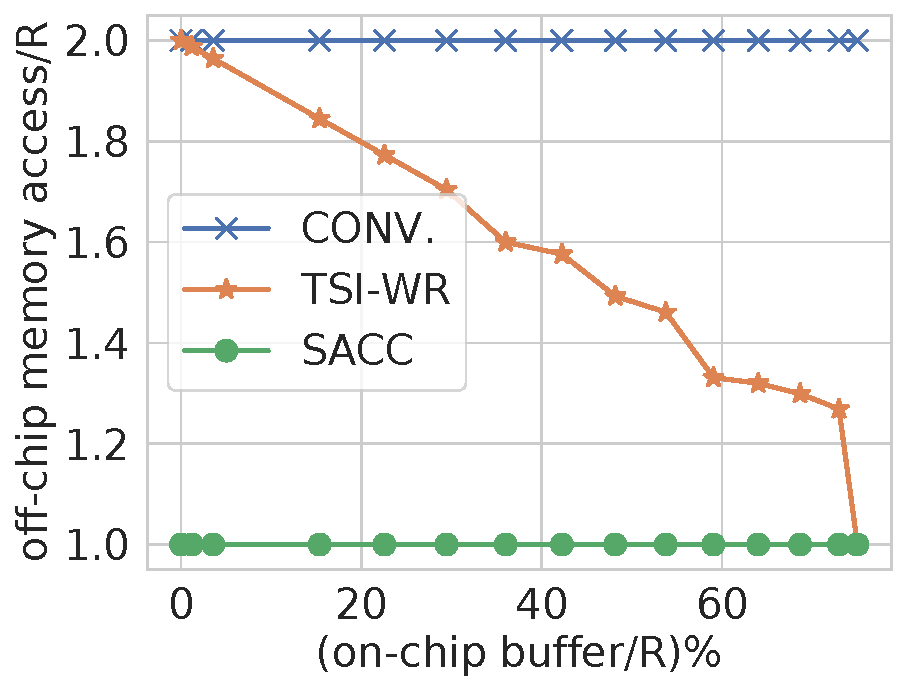
\includegraphics[width=0.35\textwidth]{tsiwrComparisonModified.pdf}
		\label{fig:memTsiwrComparison}}
	\hspace{2.0em}
	\subfloat[]
	{
		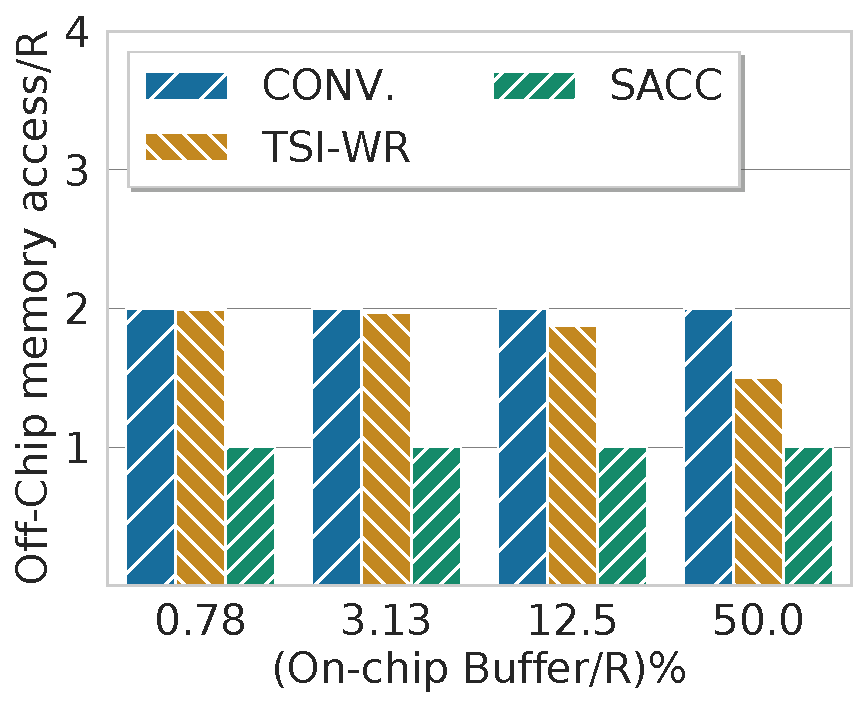
\includegraphics[width=0.35\textwidth]{memAccess2TS.pdf}
		\label{fig:memAccessAllThree}
	}
	\caption{Off-chip memory access for matrix-vector multiplication of two consecutive time steps with different on-chip buffer to R matrix size ratio.  (a)  using analytical framework (b) measured on hardware}	
	\label{fig:memAccessImprovement}
	\vspace{-1.0em}	
\end{figure}
If the on-chip buffer size is small compared to the weight matrices, tiles of R are accessed from off-chip memory replacing the older tiles in the on-chip memory. In conventional approaches, there is no reuse of these tiles for subsequent time step computations, which results in accessing full matrix $R$ every step. For conventional approaches, the off-chip memory accesses remains same, even if on chip mem size is increased as shown by the horizontal line in \figurename{~\ref{fig:memTsiwrComparison}.
The TSI-WR approach schedules the tiles in a way to reuse the data from the on-chip memory and reduces off-chip memory access. However, the extent of data reuse in the TSI-WR approach depends on the size of overlap between two consecutive tiles which is decided by the available on-chip buffer size. When the on-chip buffer to R matrix size is close to 48\%, TSI-WR reduces the memory access by $\approx$25\%, as shown in \figurename{~\ref{fig:memAccessImprovement}}. Our approach splits the computations and perform the scheduling of the tiles that reduces the memory accesses by $\approx$50\%, irrespective of the on-chip buffer size.
\subsubsection{Throughput Analysis}
\begin{figure}[htb!]
	\centering
	\subfloat[64KB on-chip buffer size]
	{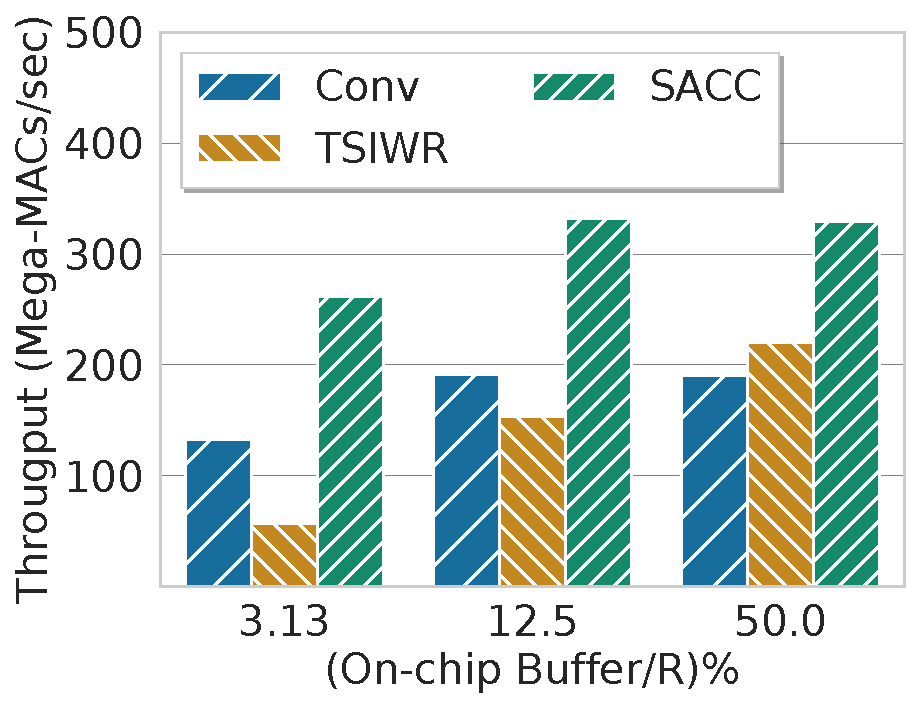
\includegraphics[width=0.35\textwidth]{througputVsMem_64KB.pdf}
		\label{fig:throughPutVsMem_64}}
	   \hspace{2.0em}
	\subfloat[128 KB on-chip buffer size]
	{
		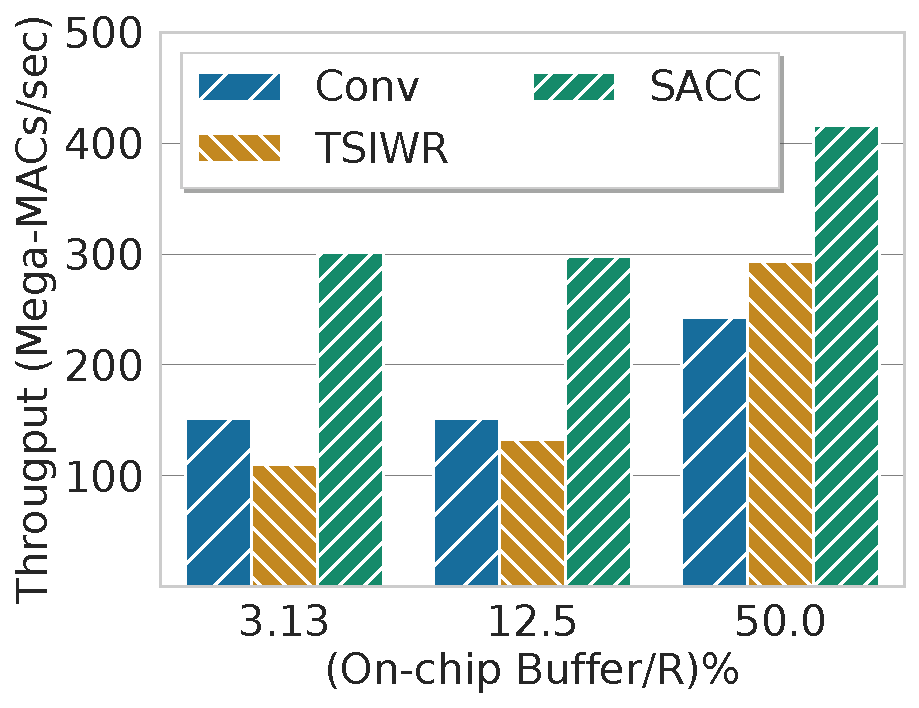
\includegraphics[width=0.35\textwidth]{througputVsMem_128KB.pdf}
		\label{fig:throughPutVsMem_128}
	}
	\caption{Throughput variation with different on-chip buffer/R ratio}	\label{fig:throughputVsMem}
\end{figure}
To analyze the throughput variation with on-chip buffer sizes, we synthesized FPGA designs with different on-chip buffer sizes for all the three approaches and measured the total run time of each design. Total number of multiply and accumlate operations (MACs) performed per output $h$ can be computed using the hidden state vector dimension ($N$) and input vector length ($L$). We measured the run times of different FPGA designs for $T$ time steps and used it to compute the throughput, as follows 
\begin{align}\label{eq:througput}
	Throughput{=}\frac{\text{Number of MACs per output}{\times}T}{\text{measured run-time}}
\end{align}
\figurename{~\ref{fig:throughPutVsMem_64}} and \figurename{~\ref{fig:throughPutVsMem_128}} compares the throughput for different ratios of on-chip buffer to weight matrix size for 64 and 128 KB on-chip buffer size, respectively.  We experimented with different number of hidden units ($N$) to vary $R$ matrix size. Increasing on-chip buffer to $R$ matrix size ratio results in larger tile sizes and fewer number of iterations, resulting in throughput improvement, for all the three approaches. The TSI-WR approach performs worse than the conventional approach for smaller on-chip buffer/$R$ ratio due to its control logic overhead which overshadows the data reuse benefits. However, for a larger on-chip buffer/$R$ size ratio (e.g., 50\%), the TSI-WR approach outperforms the conventional approach due to better data-reuse. Our approach performs better than the other two approaches for all the on-chip buffer to $R$ matrix size ratio due to its significant data-reuse of weight matrix $R$ and small control logic overhead.
For 50\% on-chip buffer to matrix size ratio, our approach improves the throughput by 42\% and 33\% for 64~KB and 41\% and 29\% for 128~KB on-chip buffer size, compared to conventional and TSI-WR approaches, respectively.
\begin{figure}[htb!]
	\centering
	\subfloat[64 KB on-chip buffer size]
	{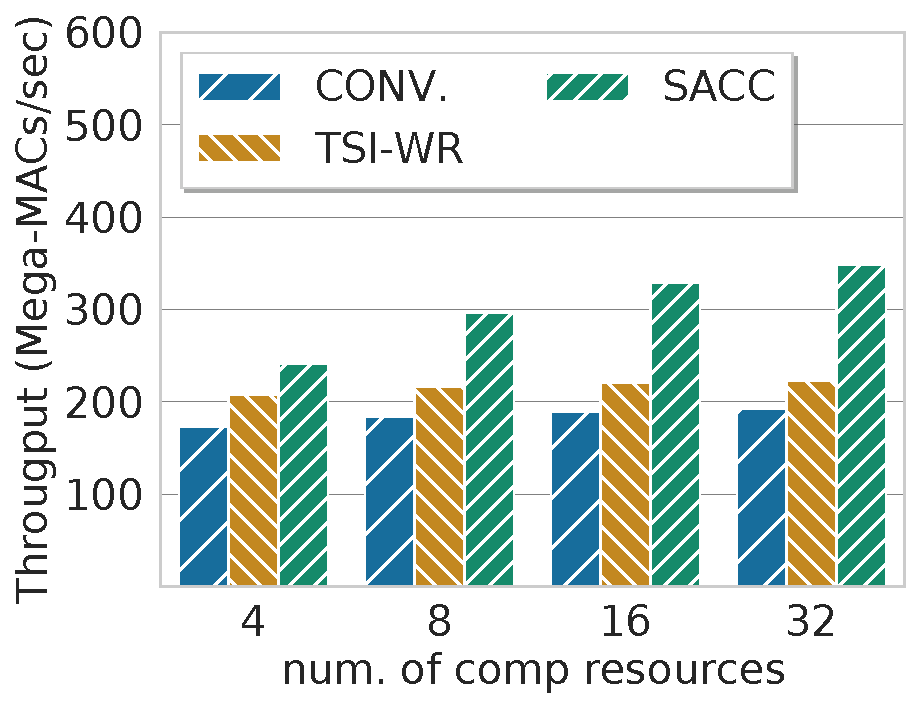
\includegraphics[width=0.35\textwidth]{througput_N128.pdf}
		\label{fig:throughPutVsPF_64}
	}
   \hspace{2.0em}
	\subfloat[128 KB on-chip buffer size]
	{
		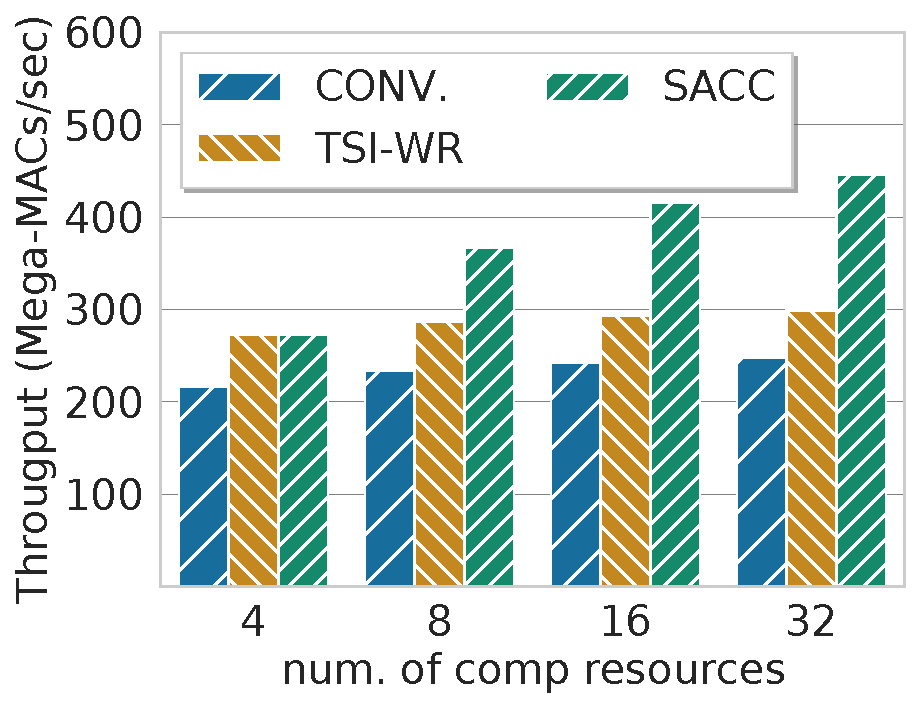
\includegraphics[width=0.35\textwidth]{througput_N256.pdf}
		\label{fig:throughPutVsPF_128}
	}
	\caption{Throughput variation of MxV with compute resources for 50\% on-chip buffer/$R$ ratio}	\label{fig:throughputVsPF}
\end{figure}
\subsubsection{Throughput variation with compute resources}
Matrix-Vector multiplication dominates the LSTM accelerators' processing. The performance of LSTM accelerators is limited by the memory bandwidth. Data reuse reduces the memory bandwidth bottleneck. To observe the impact of data reuse on memory bandwith we have implemented multiple FPGA designs with different number of compute resources, for each of the three approaches. For each approach throughput is measured using \eqref{eq:througput}. We have compared the results when on-chip buffer to matrix size ratio of 50\%. 

\figurename{~\ref{fig:throughputVsPF}} compares the throughput of the conventional, TSI-WR and our approach. 
For the conventional approach, increasing the number of computing resources does not improve the performance. TSI-WR approach improves the performance with increasing compute resources as it reuses the on-chip data and improves the operational intensity (operations/byte). However, the improvement in the TSI-WR approach is noticable only for the large on-chip buffer/$R$ size ratios. Our approach (SACC), has better operational intensity (operations/byte) and alleviates the memory bandwith issue compared to other two approaches, which results in throughput improvement with increasing the number of parallel resources. The improvement in throughput with increased number of compute resource using our approach is observed for different on-chip buffer sizes as shown in \figurename{~\ref{fig:throughPutVsPF_64}} and \figurename{~\ref{fig:throughPutVsPF_128}}.
\subsubsection{Energy Efficiency Improvement}
Using our FPGA implementations, we measured the run time for conventional, TSI-WR and SACC approaches for large number of time steps. We computed the energy consumption of the designs using the following equation~\cite{tu2017deep}
\begin{align}\label{eq:energyEfficiency}
	E~{=}~P\cdot Time~{+}~\numBytesOffChip\cdot E_{DDR}
\end{align}
where $P$ is the FPGA design power reported by the Vivado synthesis tool, $Time$ is the average run time of the design per $h$ computation, $\numBytesOffChip$ is the number of bytes accessed from off-chip memory logged using Xilinx APM IP, and $E_{DDR}$ is the off-chip memory access energy per bit. We have used $E_{DDR}$=70 pJ/bit, a typical value for the DDR3 memory access energy~\cite{6237004}.
\begin{figure}[htb!]
	\centering
	\subfloat[64KB on-chip buffer size]
	{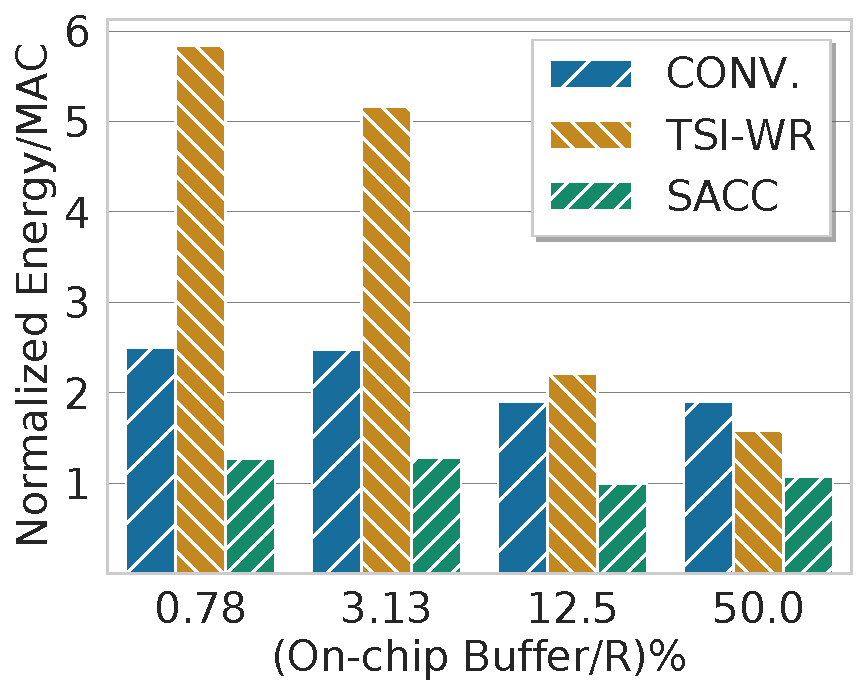
\includegraphics[width=0.35\textwidth]{energyVsMem_64KB.pdf}
		\label{fig:energy_64}
	}
	\hspace{2.0em}
	\subfloat[128 KB on-chip buffer size]
	{
		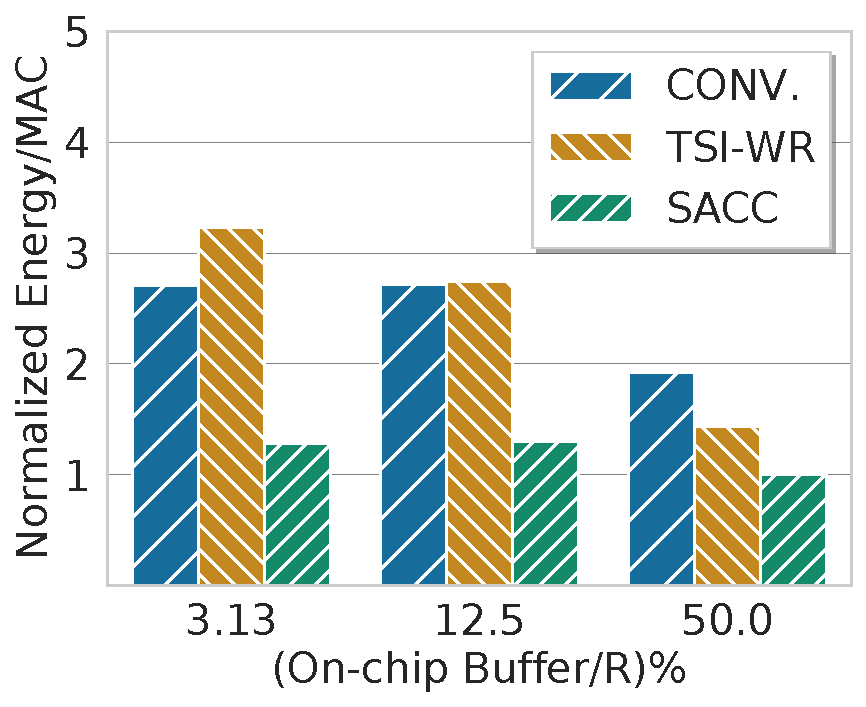
\includegraphics[width=0.35\textwidth]{energyVsMem_128KB.pdf}
		\label{fig:energy_128}
	}
	\caption{Energy improvement with on-chip buffer size/R}\label{fig:energyVsMem}
\end{figure}
\figurename{~\ref{fig:energy_64}} and \figurename{~\ref{fig:energy_128}} shows the normalized energy efficiency per MAC operation for different on-chip buffer to R matrix size ratios for 64~KB and 128~KB on-chip buffer sizes, respectively.  All three approaches observe the improvement with the increase in the on-chip buffer size to matrix size ratio due to a reduction in the control logic execution. TSI-WR performs better than the conventional approach only after on-chip buffer to R matrix size ratio is greater than 12.5\%. Our approach (SACC ) outperforms the other two approaches for all the cases as it reduces the off-chip memory accesses which dominates the overall energy consumption. For 50\% on-chip buffer to matrix size ratio, the SACC approach reduces 43\% and 32\% energy for 64~KB on-chip buffer and 48\% and 30\% for 128~KB on-chip buffer size compared to conventional and TSI-WR approach, respectively.

\section{Summary}
Long Short-Term Memory (LSTM) networks are widely used in speech recognition and natural language processing (NLP). With enormous growth in number of Edge AI applications, there is a pressing need of efficient execution of these alogrithms on edge devices. These edge devices use customized accelerators to meet the energy and throughput targets. The key to improving the energy efficiency and throughput of DNN accelerators is to reduce the off-chip memory accesses. This work proposes a novel data reuse approach that reduces the off-chip memory accesses of large weight matrices of RNNs/LSTMs by $\approx$50\% and improves the throughput significantly. Our approach improves the throughput by 55\% and 29\% and reduces the energy consumption by 52\% and 30\% for 12.5\% and 50\% on-chip buffer to matrix size ratio, for 128 KB on-chip buffer size, compared to the state of art TSI-WR approach.
